
%% 
%% Copyright 2007-2024 Elsevier Ltd
%% 
%% This file is part of the 'Elsarticle Bundle'.
%% ---------------------------------------------
%% 
%% It may be distributed under the conditions of the LaTeX Project Public
%% License, either version 1.3 of this license or (at your option) any
%% later version.  The latest version of this license is in
%%    http://www.latex-project.org/lppl.txt
%% and version 1.3 or later is part of all distributions of LaTeX
%% version 1999/12/01 or later.
%% 
%% The list of all files belonging to the 'Elsarticle Bundle' is
%% given in the file `manifest.txt'.
%% 
%% Template article for Elsevier's document class `elsarticle'
%% with numbered style bibliographic references
%% SP 2008/03/01
%% $Id: elsarticle-template-num.tex 249 2024-04-06 10:51:24Z rishi $
%%
\documentclass[preprint,12pt]{elsarticle}

%% Use the option review to obtain double line spacing
%% \documentclass[authoryear,preprint,review,12pt]{elsarticle}

%% Use the options 1p,twocolumn; 3p; 3p,twocolumn; 5p; or 5p,twocolumn
%% for a journal layout:
%% \documentclass[final,1p,times]{elsarticle}
%% \documentclass[final,1p,times,twocolumn]{elsarticle}
%% \documentclass[final,3p,times]{elsarticle}
%% \documentclass[final,3p,times,twocolumn]{elsarticle}
%% \documentclass[final,5p,times]{elsarticle}
%% \documentclass[final,5p,times,twocolumn]{elsarticle}

%% For including figures, graphicx.sty has been loaded in
%% elsarticle.cls. If you prefer to use the old commands
%% please give \usepackage{epsfig}

%% The amssymb package provides various useful mathematical symbols
\usepackage{amssymb}
%% The amsmath package provides various useful equation environments.
\usepackage{amsmath}
\usepackage{makecell}
\usepackage{multirow}
\usepackage{booktabs}% http://ctan.org/pkg/booktabs
\usepackage{xcolor}
\usepackage{graphicx}
\usepackage{sectsty}
\usepackage{longtable}
\usepackage{enumitem}
\usepackage{subcaption}
\usepackage{textcomp}
\usepackage[T1]{fontenc}
\usepackage{hyperref}

\usepackage{listings}




\newcommand{\tabitem}{~~\llap{\textbullet}~~}
\definecolor{lightgray}{gray}{0.9}
\definecolor{purple}{rgb}{0.63, 0.36, 0.94}
\definecolor{lightgreen}{rgb}{0.85, 0.92, 0.83}

% \lstdefinelanguage{SQL}{
%     keywords={SELECT, FROM, WHERE, INNER, JOIN, AS, ON, AND, IN, COUNT},
%     keywordstyle=\color{purple}\bfseries,
%     commentstyle=\color{gray}\ttfamily,
%     stringstyle=\color{blue}\ttfamily,
%     basicstyle=\scriptsize\ttfamily,
%     morecomment=[s][\color{green}]{/*}{*/},
%     morestring=[b]',
%     breaklines=true,
% }
\lstdefinestyle{prompt}{
    backgroundcolor=\color{white},
    basicstyle=\scriptsize\ttfamily,
    numbers=none,
    numberstyle=\scriptsize,
    stepnumber=1,
    numbersep=5pt,
    frame=single,
    captionpos=t,
    breaklines=true,
    breakatwhitespace=true,
    morecomment=[l]{\%},
    commentstyle=\color{red},           % 注释样式为红色
    keywordstyle=\color{black},
    stringstyle=\color{black},
    escapeinside={(*@}{@*)},
}

\lstdefinestyle{my_operation}{
    basicstyle=\scriptsize\ttfamily,
    keywordstyle=[1]\color{red},        % Tool 关键字颜色为红色
    keywordstyle=[2]\color{orange},     % Thought 关键字颜色为橙色
    keywordstyle=[3]\color{blue},     % Blue 关键字颜色为橙色
}
% 定义三个分类的关键字
% \lstset{
%     style=my_operation,
%     morekeywords=[1]{SQL},  % SQL 关键词
%     morekeywords=[2]{Tool},                          % 
%     morekeywords=[3]{Thought}                  % Thought 关键词
% }

\lstdefinestyle{sql_command}{
    basicstyle=\scriptsize\ttfamily,
    % keywordstyle=[1]\color{blue},       % SQL 关键字颜色为蓝色
    % keywordstyle=[2]\color{red},        % Tool 关键字颜色为红色
    % keywordstyle=[3]\color{orange},     % Thought 关键字颜色为橙色
}
\lstset{
    % style=sql_command
    % style=my_operation,
    % language=SQL,
    backgroundcolor=\color{lightgray},
    extendedchars=true,
    basicstyle=\scriptsize\ttfamily,
    showstringspaces=false,
    showspaces=false,
    tabsize=2,
    breaklines=true,
    breakatwhitespace=false,
    frame=lines,
    moredelim=[is][\bfseries\color{purple}]{@}{@},
    aboveskip=-12pt,
    belowskip=-12pt,
    moredelim=[is][\bfseries\color{brown}]{~}{~},
    morekeywords=[1]{Tool},                          % 
    morekeywords=[2]{Thought},
    morekeywords=[3]{SQL}  % SQL 关键词
}

%% The amsthm package provides extended theorem environments
%% \usepackage{amsthm}

%% The lineno packages adds line numbers. Start line numbering with
%% \begin{linenumbers}, end it with \end{linenumbers}. Or switch it on
%% for the whole article with \linenumbers.
%% \usepackage{lineno}

\journal{Jounal of Manufacturing System}

\begin{document}

\begin{frontmatter}

%% Title, authors and addresses

%% use the tnoteref command within \title for footnotes;
%% use the tnotetext command for theassociated footnote;
%% use the fnref command within \author or \affiliation for footnotes;
%% use the fntext command for theassociated footnote;
%% use the corref command within \author for corresponding author footnotes;
%% use the cortext command for theassociated footnote;
%% use the ead command for the email address,
%% and the form \ead[url] for the home page:
%% \title{Title\tnoteref{label1}}
%% \tnotetext[label1]{}
%% \author{Name\corref{cor1}\fnref{label2}}
%% \ead{email address}
%% \ead[url]{home page}
%% \fntext[label2]{}
%% \cortext[cor1]{}
%% \affiliation{organization={},
%%             addressline={},
%%             city={},
%%             postcode={},
%%             state={},
%%             country={}}
%% \fntext[label3]{}

\title{
% Chat with MES - A Case Study of Garment Manufacturing System.
Chat with MES: LLM-driven User Interface for Manipulating Garment Manufacturing System through Natural Language
}

%% use optional labels to link authors explicitly to addresses:
%% \author[label1,label2]{}
%% \affiliation[label1]{organization={},
%%             addressline={},
%%             city={},
%%             postcode={},
%%             state={},
%%             country={}}
%%
%% \affiliation[label2]{organization={},
%%             addressline={},
%%             city={},
%%             postcode={},
%%             state={},
%%             country={}}

\author[ustb,ise]{Zhaolin Yuan} %% Author name
\author[ise,riam,rcdt,transgp]{Ming Li\corref{cor1}} %% Author name
\author[ustb]{Chang Liu} %% Author name
\author[ustb]{Fangyuan Han} %% Author name
% \ead{julian.yuan@polyu.edu.hk}
\author[jnu]{Haolun Huang} %% Author name
% \ead{julian.yuan@polyu.edu.hk}
\author[hkbt]{Hong-Ning Dai} %% Author name

\cortext[cor1]{Corresponding author}

%% Author affiliation
\affiliation[ustb]{organization={Institute of Artificial Intelligence, University of Science and Technology Beijing},
            city={Beijing},
            country={China}}
\affiliation[ise]{organization={Department of Industrial and Systems Engineering, the Hong Kong Polytechnic University },%Department and Organization
            % addressline={}, 
            city={Hong Kong},
            country={China}}
\affiliation[riam]{organization={Research Institute of Advanced Manufacturing, the Hong Kong Polytechnic University},%Department and Organization
            % addressline={}, 
            city={Hong Kong},
            country={China}}
\affiliation[rcdt]{organization={Research Centre for Digital Transformation of Tourism, The Hong Kong Polytechnic University, Hung Hom},
            city={Hong Kong},
            country={China}}
\affiliation[transgp]{organization={Centre for Transformative Garment Production,  Hong Kong Science Park, Pak Shek Kok},
city={Hong Kong},
country={China}}
\affiliation[hkbt]{organization={Department of Computer Science, Hong Kong Baptist University},%Department and Organization
            % addressline={}, 
            city={Hong Kong},
            country={China}}
            % H.-N. Dai is with the Department of Computer Science, Hong Kong Baptist University, Hong Kong (e-mail: hndai@ieee.org). 
\affiliation[jnu]{organization={School of Intelligent Systems Science and Engineering, Jinan University},%Department and Organization
            % addressline={}, 
            city={Zhuhai},
            country={China}}
%% Abstract
\begin{abstract}
%% Text of abstract
% Abstract text.

This paper presents Chat with MES (CWM), an AI agent system, which integrates LLMs into the Manufacturing Execution System (MES), serving as the "ears, mouth, and the brain". 
This system promotes a paradigm shift in MES interactions from Graphical User Interface (GUI) to natural language interface", offering a more natural and efficient way for workers to manipulate the manufacturing system.
Compared with the traditional GUI, both the maintenance costs for developers and the learning costs and the complexity of use for workers are significantly reduced.
This paper also contributes two technical improvements to address the challenges of using LLM-Agent in serious manufacturing scenarios.
The first one is Request Rewriting, designed to rephrase or automatically follow up on non-standardized and ambiguous requests from users.
% which enhances understanding and pre-processing of non-standardized and ambiguous user inputs by pre-identifying common entities in manufacturing, such as customers, products, and materials.
The second innovation is the Multi-Step Dynamic Operations Generation, which is a pre-execution planning technique similar to Chain-of-Thought (COT), used to enhance the success rate of handling complex tasks involving multiple operations.
% . It is a approximated to Chain of Thought
% The second innovation is Multi-Step Dynamic Operations Generation, which decomposes a complex request into a sequence of simple operations, such as executing an SQL command or invoking a tool. 
A case study conducted on a simulated garment MES with 55 manually designed requests demonstrates the high execution accuracy of CWM (80\%) and the improvement achieved through query rewriting (9.1\%) and Multi-Step Dynamic operations generation (18.2\%). 
The source code of CWM, along with the simulated MES and benchmark requests, is publicly accessible.


\end{abstract}

%%Graphical abstract
% \begin{graphicalabstract}
% %\includegraphics{grabs}
% \begin{figure}[h]
%     \centering
%     \includegraphics[width=\linewidth]{figs/.pdf}
%     \caption{Caption}
%     \label{fig:enter-label}
% \end{figure}
% \end{graphicalabstract}

%%Research highlights
\begin{highlights}
\item An LLM-agent system, named "Chat with MES" (CWM), is proposed to replace the graphical user interface in the MES and enable human-computer interaction via linguistic commands.
\item 
For enhancing the controllability and reliability of the LLM and incorporating prior production guidelines,
the Multi-step Dynamic Operations Planning and Execution is proposed to break down the intricate task as a chain of controllable and atomic operations.
\item 
To assess the CWM as the human-MES interface, 
we build a brand-new benchmark, including a garment manufacturing system with simulated data and 55 manually crafted requests and labeled ground-truths.
\item The CWM exhibits a commendable execution success rate of 80\%, surpassing the performance of the original GPT-4, which records a success rate of 60\%.
% The improvement ensures the controllability and reliability of CWM in serious manufacturing scenarios.
% \item 
% A brand-new simulation of production data within a small garment manufacturing system was implemented. 

% To address the limitations of general LLMs in handling complex tasks that require strong prior knowledge, this study introduces the Multi-step Dynamical Operation Generation technique, which guides large language models (LLMs) in decomposing a complex task into a series of basic executable operations. With this technique, the execution accuracy of CWM in handling complex requests is improved by over 18\%, reaching 80\%.
\end{highlights}

%% Keywords
\begin{keyword}
Interactive Manufacturing Execution System, Large Language Model, Text2SQL, LLM-Agent, Human-Computer Interaction.
%% keywords here, in the form: keyword \sep keyword

%% PACS codes here, in the form: \PACS code \sep code

%% MSC codes here, in the form: \MSC code \sep code
%% or \MSC[2008] code \sep code (2000 is the default)

\end{keyword}

\end{frontmatter}

%% Add \usepackage{lineno} before \begin{document} and uncomment 
%% following line to enable line numbers
%% \linenumbers

%% main text
%%

%% Use \section commands to start a section
\section{Introduction}

The Manufacturing Execution System (MES) has undergone significant evolution since its inception in the late 19th century, becoming an integral part of modern manufacturing due to its crucial role in production process management and optimization~\cite{doi:10.1080/09537280902938613}. 
With the rapid development of MES in incorporating more complicated functions and operational workflows, the methods by which workers interact with MES warrant more attention~\cite{9781176}. 
Efficient and friendly interaction will significantly reduce the workload of workers and the training cost for new employees.

% Despite its importance, MES faces several challenges, particularly in environments where production processes are complex and involve intricate logic.

Since the Graphical User Interface (GUI) appeared~\cite {martinez2011graphical}, 
it has become the primary way for workers to operate an MES.
% it the primary way through which workers operate an MES is the .
Users manipulate the graphical elements within a specific system page and receive feedback from the changeable elements.
The GUI is typically developed alongside the core components of the MES by the software engineering team.
Although the GUI in has evolved over several decades and is sufficiently mature, it still suffer some limitations in real developments and utilization.
% Although the frameworks for developing GUI, including web pages and application pages, have evolved over several decades 
The first limitation arises from the programmers responsible for coding.
% Developing and maintaining an MES, as a non-standardized and customized software, demands substantial labor effort.
Because MES is a kind of non-standardized and customized software, it demands substantial labor effort for developing and maintaining the GUI.
Even after project delivery, users may still present various new requirements and the developers have to intervene and revise the logic of software and data access interfaces.
Many MES development projects fail and are abandoned by factory users because the development team refuses to continue maintaining the systems~\cite{pr10112173}.
The second issue is the learning cost and operational complexity for users.
A new worker must thoroughly learn from the software guidelines and undergo training before performing operations.
In the utilization stage, the workload is also significant due to numerous repetitive and tedious operations.
For systems designed for extremely complicated manufacturing processes, the cost for developing and using GUI is much more substantial~\cite{li2022application}.

% Literature Review
Advanced software engineering methods are suggested to address challenges in development and implementation. 
From the perspective of reducing the labor cost of software development and maintenance,
emerging software development techniques have explored paradigms such as no-code~\cite{rokis2022challenges} and low-code~\cite{cabot2020positioning} development platforms.
However, these platforms face usability--plasticity dilemma.
% High cost of learning new software and frameworks.
% The major one is the trade-off between usability and extensibility. 
Component encapsulation allows non-programmers to swiftly create a software system through drag-and-drop interfaces.
However, excessive encapsulation will adversely affect extensibility, making it impossible to meet customized needs.
From a worker's experience standpoint in relation to usage, Robotic Process Automation (RPA)\cite{siderska2020robotic} has garnered substantial interest as a means of automating repetitive and labor-intensive business processes through software bots.
However, the functions of most RPA engines are generally limited to specific workflows and certain GUI pages.
They merely serve as supplemental tools to the GUI rather than substitutes for addressing the underlying drawbacks of GUI.
% When the platform cannot meet the user's customized needs, embedding natively developed pages becomes very challenging.

Recent advances in large language models (LLMs) have the potential to revolutionize the interaction between humans and information systems.
%======================================================================
% 第一篇引用
%The rapid spread of AI applications makes it necessary to develop new approaches for future Human-Computer interfaces, which differ from classical interfaces due to AI's human-like cognitive, self-executing, and self-adapting capabilities~\cite{holzinger2022personas}.
%======================================================================
This can be achieved by understanding the user requirements expressed in natural language and invoking the services within the information system.
Some successful cases have been observed in Web Shopping~\cite{yao2022webshop} and Web Browsing\cite{deng2024mind2web}.
% As a typical information system, MES can be accessed by large language models (LLMs), allowing us to equip it with a conversational interface as the user interface.
%=======================================================================
% 第二篇引用
%Trust can be achieved through counterfactual explanations, which allow people to familiarize themselves with unknown processes by understanding the hypothetical input conditions under which the outcome changes~\cite{delser2024counterfactual}. This approach is particularly important for enhancing the reliability and trustworthiness of AI systems in critical applications.
%========================================================================
Accessing an MES through a conversational interface powered by an LLM is straightforward. 
However, manufacturing is a typical serious and complicated scenario.
It introduces two technical challenges when utilizing LLMs to manipulate a MES.
First, in terms of user input, the inherent flexibility of natural language often leads to ambiguity in user input~\cite{yadav2021comprehensive}. 
% It conflicts with the requirement for precise instructions necessary to ensure reliable MES operations.
It contradicts the need for precise instructions, which are essential for reliable operations in MES.
An important research topic is enabling LLM systems to identify accurate information from incorrect or ambiguous queries.
From the perspective of handling a request, a user request may involve numerous database operations and service calls, presenting a challenge for existing large language models (LLMs) to accurately execute all steps.
% which are beyond the current intellectual capabilities of LLMs.
Manufacturing is a serious application domain and many operations involve atomicity and transactional properties. 
For the LLM Agent, the procedure for processing requests and the operations it executes have to be governed by pre-established factory management guidelines. 
Inaccurate operations can lead to severe consequences.
These two issues must be addressed before using an LLM-based interface to manipulate the real MES.
% The second research question this paper focusing is about 

% leading to over-reliance on human knowledge and losing generalization across various manufacturing scenarios.
% The need for absolutely accurate instructions to ensure reliable MES operations conflicts with the inherent ambiguity of natural language, where user inputs often contain ambiguities.

% through conversational interfaces and executing corresponding commands. 
% This transformation is evident in three key areas:

% Knowledge-based Q\&A.
% LLM agents acting as API callers and SQL generators.
% LLMs functioning as transactional mediators.
% However, leveraging LLMs to transform the use of MES systems presents significant challenges:

% Manufacturing is a critical application domain where inaccurate information or generative hallucinations by LLMs can have dire consequences.
% Simple user requests in an MES context often necessitate a series of complex system operations, beyond the current intellectual capabilities of LLMs, leading to over-reliance on human knowledge and losing generalization across various manufacturing scenarios.
% The need for absolutely accurate instructions to ensure reliable MES operations conflicts with the inherent ambiguity of natural language, where user inputs often contain ambiguities.
\begin{figure}[t]
    \centering
    \begin{subfigure}{\textwidth}
    \centering
    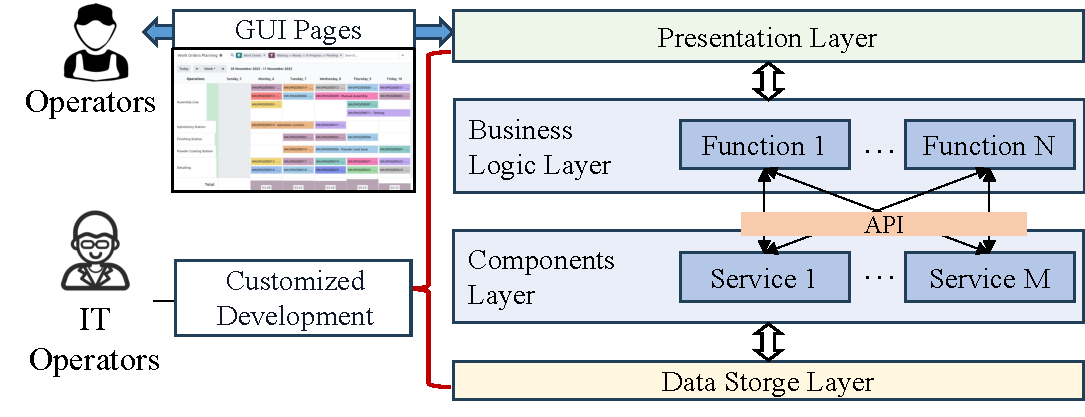
\includegraphics[width=0.8\linewidth]{figs/MES.pdf}
    \caption{Framework of Traditional GUI-based MES.}
  \end{subfigure}

  \begin{subfigure}{\textwidth}
    \centering
    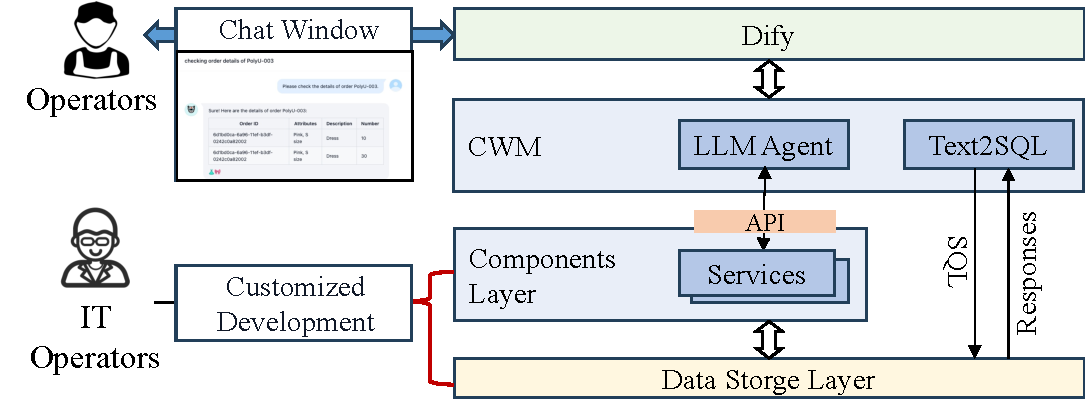
\includegraphics[width=0.8\linewidth]{figs/CWM.pdf}
    % \caption{Chat with MES: Operating MES via Natural Language.}
    \caption{New paradigm for operating MES via CWM.}
  \end{subfigure}
    \caption{The comparison between the traditional GUI-based framework and CWM.}
    \label{fig:cmp_MES_CWM}
\end{figure}

% The paper proposes 
This paper presents a system entitled "Chat with MES" (CWM) to replace the traditional GUI of MES with conversational interactions.
%=========================================================================
%In the context of designing such human-AI interfaces for various heterogeneous groups of people, appropriate methodological approaches are required.
%Personas are very important in the context of human-centered development because they map the mental models of users to specific contexts.
%The rapid spread of AI applications makes it necessary to develop new approaches for future human-AI interfaces, which differ from classical human-computer interfaces due to AI's human-like cognitive, self-executing, and self-adapting capabilities~\cite{holzinger2022personas}.
%=========================================================================
% This manuscript presents a platform entitled "Chat with MES" (CWM) that is specifically developed to supplant the conventional graphical user interface of Manufacturing Execution Systems (MES) with conversational interactions. Figure
Figure~\ref{fig:cmp_MES_CWM} presents the differences between using CWM and traditional GUI to manipulate MES.
The CWM obviates the necessity for developing both front-end and back-end software, in addition to reducing the expenses associated with system maintenance.
Furthermore, we propose two technical advancements to address the challenges associated with ambiguous user inputs and complicated tasks.
\textbf{1) Query Rewriting}: This module addresses the problem of ambiguous and inaccurate user inputs by maintaining a private context base to record named entity information and rewrite users' requests. 
% Additionally, it employs multi-turn dialogues to gather more information and eliminate ambiguities.
\textbf{2) Multi-step Dynamic Operations Planning and Execution}: 
% To best handle complicated users' requests, we combine the Text2SQL and LLM-Agent to generate and execute operations dynamically based on a pre-defined basic operations tool and a relational database. 
% The original task is decomposed as a series of basic operations.
% Each operation corresponds to either invoking a service in the MES or directly generating an SQL command to access the database.
To effectively handle complicated user requests, the Multi-step Dynamic Operations Planning and Execution pre-plans a chain of basic executable operations with parameter placeholders and execute the operations one-by-one.
Each operation involves either invoking a service from the MES's predefined services pool, generating an SQL command for direct access to the production database, or performing reasoning and inference based on context.
The initial decomposition significantly enhances the controllability and reliability of the LLM and facilitates the incorporation of prior knowledge.
%======================================================================
%Trust can be achieved through counterfactual explanations, which allow people to familiarize themselves with unknown processes by understanding the hypothetical input conditions under which the outcome changes~\cite{delser2024counterfactual}. This approach is particularly important for enhancing the reliability and trustworthiness of AI systems in critical applications.
%======================================================================
We evaluated the CWM on a simulated garment MES and a manually designed questions-and-answers dataset involving 55 requests.
The garment manufacturing execution system (MES) is equipped with a relational database consisting of 16 tables, encapsulating the typical components encountered in actual garment production.
The designed requests encompass the major cases that may arise during actual use by the two user roles: workers, and managers.
% involving common questions and operation .
The quantitative findings indicate a high execution accuracy of the CWM at 80\%, along with the enhancement achieved through query rewriting, which contributes an improvement of 9.1\%, and the generation of Multi-Step Dynamic operations, which results in an advancement of 18.2\%.
% All operational plans are dynamically generated based on the responses from the preceding operation step.

% The differences between using CWM and traditional GUI to manipulate MES are shown in Figure~\ref{fig:cmp_MES_CWM}.

% To manage the complexity of MES business processes, 

% this stage decomposes intricate problems into manageable steps through dynamic SQL generation.

The contributions of this paper are threefold.

1) We propose "Chat with MES," a novel MES operation paradigm that provides users with an interface for manipulating the MES system via natural language.

2) The Multi-step Dynamical Operations Generation is proposed to handle complex user queries by executing a sequence of basic operations. This technique ensures the controllability and reliability of CWM in serious manufacturing scenarios.

3) An experimental environment was established using a simulated garment manufacturing system. Furthermore, a new question-and-answer dataset comprising 55 manually crafted queries was created to serve as a new benchmark for operating a Manufacturing Execution System (MES) through conversation.  
The evaluation of the CWM demonstrates an impressive execution success rate of 80\%, significantly exceeding the original GPT-4's performance, which registers at 60\%.

The subsequent sections are organized as follows:
Section~\ref{sec:related_work} provides a review of existing literature concerning user interfaces within Manufacturing Execution Systems (MES), as well as the application of Large Language Models (LLM) in manufacturing processes and techniques associated with LLM.
Section~\ref{sec:method} depicts the technical details of CMS including the Query Rewriting and Multi-step Dynamical Operations Generation.
% The experimental Section~\ref{sec:exp} introduces the testing garment manufacturing system and the Q/A dataset. 
The experiment Section~\ref{sec:exp} provides an introduction to the simulated garment manufacturing system used for testing, along with the corresponding Q/A dataset.
Next, the experimental results and analysis are presented.
Section \ref{sec:discussion} discusses the limitations of CWM and provides insight into future research. 
Finally, Section \ref{sec:conclusion} concludes this article.


\section{Related Work}
\label{sec:related_work}
\subsection{Limitations in Human-MES interaction}
% Because of the many distinct elements of MES, 
An integrated management interface is indispensable for each MES to ensure that the distinct components are systematically organized and accessible.
Graphical user interface (GUI) serves to convey information to users and facilitate human decision-making in production management~\cite{SHOJAEINASAB2022503}. 
This section examines recent research concerning the creation and utilization of GUI. 

% Advanced software engineering methods are suggested to address challenges in development and implementation. 
% From the perspective of reducing the labor cost of software development and maintenance,
% emerging software development techniques have explored paradigms such as no-code~\cite{rokis2022challenges} and low-code~\cite{cabot2020positioning} development platforms.
% However, these platforms face usability--plasticity dilemma.
% % High cost of learning new software and frameworks.
% % The major one is the trade-off between usability and extensibility. 
% Component encapsulation allows non-programmers to swiftly create a software system through drag-and-drop interfaces.
% However, excessive encapsulation will adversely affect extensibility, making it impossible to meet customized needs.
% From a worker's experience standpoint in relation to usage, Robotic Process Automation (RPA)\cite{siderska2020robotic} has garnered substantial interest as a means of automating repetitive and labor-intensive business processes through software bots.
% However, the functions of most RPA engines are generally limited to specific workflows and certain GUI pages.
% They merely serve as supplemental tools to the GUI rather than substitutes for addressing the underlying drawbacks of GUI.
% From the development perspective, manufacturing is a customized scenario, leading the transaction logic and GUI have to be customized for each individual factory.
In development terms, manufacturing is a tailored scenario, requiring customization of transaction logic and the GUI for each factory.
To address the significant cost associated with customized development, many software development techniques have explored paradigms such as no-code~\cite{rokis2022challenges} and low-code~\cite{cabot2020positioning} development platforms.
% In spite of the maturity of GUI development frameworks, limitations persist in MES development due to the substantial labor required for customization and maintenance.
% , coupled with high learning costs and operational complexity for users.
% Low-code ~\cite{cabot2020positioning} and no-code~\cite{rokis2022challenges} development are recent trends that
These platforms integrate tools for a specific kind of applications and enable end developers to create and configure corresponding applications by themselves, such as ERP, MES, and digital twin systems~\cite{DALIBOR2022101117}.
Although these techniques are known to be easily developed, deployed, and maintained, they nevertheless face limitations in extensibility, rendering them unsuitable for complicated manufacturing scenarios~\cite{rokis2022challenges}.

In the utilization perspective, intricate manufacturing systems are associated with significant learning expenses and operational complexities for users.
As a revolutionary technique to simplify the operational processes and enhance user experience, Robotic Process Automation (RPA)~\cite{siderska2020robotic} has garnered substantial interest as a means of automating repetitive and labor-intensive business processes through software bots.
% SmartFlow integrates computer vision and LLMs to automatically generate navigation workflows and adapt to variations in GUIs and applications without human intervention~\cite{jain2024smartflow}.
% Wang et al.\cite{wang2023enabling} conducted a study exploring the use of pre-trained language models (LLMs) to enable conversational interaction on mobile user interfaces (UIs)
Recent work by Holzinger et al. ~\cite{holzinger2022personas} highlights the importance of human-centered Artificial intelligence (AI) interfaces.
Current RPA systems are most designed to adhere to pre-defined rules and workflows of the GUI~\cite{jain2024smartflow}.
These functionalities are typically implemented through drag-and-drop interfaces, screenplay recording, or automation frameworks such as Selenium~\cite{sharma2014web}.
The systems are intrinsically system-centered, instead of human-centered.
Users must passively adhere to the rules and provide specific information, yet they cannot actively express their desires~\cite{jain2024smartflow}.
Meanwhile, RPA remains dependent on GUI interfaces, the cost of developing GUI is unavoidable.
Recent years have witnessed remarkable progress in computer vision, LLM, and LLM-Agent, which have opened up new possibilities for integrating LLMs with RPA systems towards enabling them to perceive and autonomously interact with complex applications.
% The system is fundamentally centered around itself rather than the user. Users must adhere to set regulations and supply precise data, yet they lack the ability to actively convey their desires.
% , particularly in domains where explainability and causability are crucial. 
AI can be incorporated into the interface layer for MES to create better user-friendly experiences. 
Mantravadi et al.~\cite{mantravadi2020user} proposed the concept of AI-based chatbot assistance, which aims at production coordination by assisting the shop floor workforce and providing easy information
extraction in manufacturing.
Their developed prototype shows that MES users can benefit from an interactive chatbot by creating more dynamic and free experiences.
Colabianchi et al.~\cite{colabianchi2023human} presented an integrated conceptual architecture to develop industrial conversational agents and illustrated the elements needed for the development. 
They also overlooked the application of LLMs in manufacturing conversation systems.
The research discussed above primarily stays at the conceptual or prototype development stage. 
A significant gap exists between the conceptual design and the development of a fully operational conversational system.

\subsection{LLM-based Text2SQL}
One primary function of MES is managing the production data by accessing the production databases. 
To address the wide range of potential queries from users, the proposed CWM will act as a database operating agent between the user and the database. 
Text2SQL parsing~\cite{li2024codes} aims at converting natural language questions into executable SQLs. 
Recent advances in large language models (LLMs), such as GPT-4 and Claude-2 have shown impressive results in this task. Some production-ready projects are also developed, such as DB-GPT~\cite{xue2023dbgpt} and sqlcoder~\footnote{https://github.com/defog-ai/sqlcoder}.
However, according to the test results from a large-scale Text2SQL benchmark, the most effective Text2SQL models achieve 54.89\% in execution accuracy, whereas human experts achieve approximately 92.96\%~\cite{li2024can}. 

Intrinsically, Text2SQL is a code generation technology that transforms detailed and precise natural language requests into SQL commands. 
In practical applications, it must incorporate business-related prior knowledge alongside Text2SQL to accurately identify users' requirements and generate executable SQL commands.
By designing specific workflows and incorporating additional knowledge through prompt engineering, the performance of Text2SQL in practical applications has been improved significantly. 
As an extension of Text2SQL, ChatBI is proposed to convert Natural Language to Business Intelligence~\cite{lian2024chatbi}, effectively addressing challenges related to a large number of columns. 
To address complex queries requiring multi-step database operations rather than a single SQL command, ChatDB~\cite{hu2023chatdb} and Din-SQL~\cite{pourreza2024din} augment LLMs to generate multi-step and dynamical SQL instructions for database manipulation. 
However, existing LLM-based business intelligence systems are generally applied in non-intrusive data query scenarios to avoid the catastrophic consequences of hallucinatory data editing.
In our study, manipulating MES inevitably involves a number of update, insert, and delete operations. 
The chosen operations and their order must be absolutely accurate. 
This places extremely high requirements on the agent. 
Not only does the agent need to understand all database's schemas and their relationships, but it also needs to follow the production guidelines.
% As a fundamental technology, Text2SQL is still distant from enabling conversational interactions with real Manufacturing Execution System (MES) databases. 
% Within the operational framework of a Manufacturing Execution System (MES), addressing user requests entails the complex task of dataset record manipulation, which proves to be significantly more challenging.



% However, by designing specific workflows and incorporating additional prior knowledge through prompt engineering,  the performance of Text2SQL in practical applications has been improved significantly. As an extension of NL2SQL, the ChatBI is proposed to convert Natural Language to Business Intelligence~\cite{lian2024chatbi}, effectively addressing challenges related to limited interaction modes and a large number of columns. 


% \subsection{LLM Agent}
% LLM has become an ideal foundation model for advancing AI agents toward broad and versatile functionality \cite{DBLP:conf/iclr/0036YZXLL0DMYZ024}. 
% An LLM agent takes charge of a defined set of tools, each accompanied by a textual description delineating its functionality and input/output parameters, with an LLM performing the role of the scheduler. 
% Given a complex problem, the LLM generates the plan via Chain-of-Thought~\cite{wei2022chain} and sequentially invokes approximate tools with parameters extracted from the context. 
% In manufacturing, most systems provide standardized API and protocols for integrating with other software~\cite {SHOJAEINASAB2022503}. 
% Functioning as a mediator between human operators and the MES, the CWM needs to engage with the MES through these pre-established APIs. 
% For integration of the LLM into serious and complicated manufacturing contexts, it is crucial that the agent's inferences and behaviors are transparent, explainable, and controllable~\cite{delser2024counterfactual}.

% Recent advancements in explainable AI (XAI) have shown that LLMs can be used to generate trustworthy counterfactual explanations~\cite{delser2024counterfactual}.

% The study introduces the LLM-Agent to invoke MES tools and services automatically.
% Recent advancements in explainable AI (XAI) have shown that LLMs can be used to generate trustworthy counterfactual explanations, which are crucial for understanding the decision-making processes of AI systems in high-stakes domains such as manufacturing~\cite{delser2024counterfactual} .


\subsection{Application of LLM in Manufacturing systems}
In the context of Industry 4.0, the rapid emergence of LLM has brought forth transformative solutions for manufacturers in processing and leveraging their data efficiently. 
LLMs are increasingly being used as conversational agents, serving as an intuitive interface between humans and the manufacturing environment~\cite{colabianchi2023human}. 
This section aims to analyze the differences between this paper and other studies that apply large models in the manufacturing scenarios.
% This integration enables seamless communication between operators and machines, bridging cognitive gaps and fostering real-time decision-making 
Sun et al. ~\cite{sun2024empowering} propose an AI-driven digital-twin (DT) multi-agent architecture powered by LLMs to enhance equipment maintenance scenarios, offering novel insights into predictive and preventive maintenance strategies. 
% This kind of intelligence-driven architecture facilitates more efficient predictive maintenance frameworks and data-driven asset management within industrial ecosystems.
Furthermore, the application of LLMs extends beyond conversational agents and into more specialized areas such as robotics programming. In a ROS (Robot Operating System) environment, Xia et al. demonstrate how LLM-driven code generation can be harnessed to enable more efficient robot operations~\cite{XIA2024102728}. 
% This use of LLMs in dynamic programming environments showcases AI’s ability to optimize and speed up traditionally time-consuming processes, highlighting its remarkable potential in enhancing operational efficiency.
Li et al.~\cite{li2024building} further explore the integration of LLMs with Knowledge Graphs, leveraging the symbiotic relationship between these technologies to aid in sourcing and identifying smaller manufacturing partners. 
% By interfacing with ChatGPT, manufacturers can query expansive data sets to pinpoint potential collaborators, thereby increasing flexibility and agility within supply chains.
Additionally, Xu et al.~\cite{xu2024llm} incorporate LLMs in collaborative design processes where LLMs generate design prompts for tools like DALL-E, facilitating the rapid and seamless creation of precise visual schemes.
In the realm of industrial sustainability, Wu introduces the ProcessCarbonAgent framework, which uses LLMs to analyze root causes of carbon emissions and improve decision-making for industrial emission management~\cite{wu2024processcarbonagent}. 
% This innovative system exemplifies the application of LLMs in environmental management, providing manufacturers with AI-driven insights to meet ever-increasing sustainability goals. 
These studies illustrate the transformative influence LLMs hold within numerous aspects of manufacturing, ranging from robot manipulation and design collaboration to supply chain enhancement and cause analyses.
The LLM functions not only as a chatbot or writer but also as a coordinator that integrates services and processes information from multiple sources.
Table~\ref{tab:comparison} highlights the differentiating factors of CWM in comparison to preceding research efforts. 
Given that each related work addresses unique research questions, we analyze the capabilities of LLMs that are employed. 
CWM represents the first dialogue-oriented open-source framework endowed with functionalities including Code Generation, database access, and Tool invocation.


\begin{table}[t]
\centering
\caption{Comparison of LLM-based applications in the field of manufacturing.}
\label{tab:comparison}
\resizebox{\textwidth}{!}{
\begin{tabular}{ l |c| c | c | c | c | c }
\hline
Objective&\multicolumn{1}{c|}{\textbf{Ref}}                                          & \textbf{Chat} & \textbf{\makecell[c]{Text \\Generation}} & \textbf{\makecell[c]{Code \\Generation}} & \textbf{\makecell[c]{SQL \\Generation}} & \textbf{\makecell[c]{Tool \\Invocation}} \\ 
\hline
           Conversational chatbot&\cite{colabianchi2023human}                     & $\checkmark$      & $\times$                & $\times$                & $\times$               & $\times$                \\ 
\hline
           Equipment maintenance&\cite{sun2024empowering}                        & $\times$          & $\checkmark$            & $\times$                & $\times$               & $\times$                \\ 
\hline
                \makecell[l]{Answering queries \&\\ generating robot code}&\cite{XIA2024102728}   & $\checkmark$      & $\times$                & $\checkmark$            & $\times$               & $\times$                \\ 
\hline
\makecell[l]{Manufacturing \\service discovery}&\cite{li2024building}            & $\checkmark$      & $\times$                & $\times$                & $\checkmark$           & $\times$                \\ 
\hline
Collaborative design&\cite{xu2024llm}                       & $\checkmark$      & $\checkmark$            & $\times$                & $\times$               & $\times$                \\ 
\hline
 \makecell[l]{Carbon emission \\management}&\cite{wu2024processcarbonagent}                 & $\checkmark$      & $\checkmark$            & $\times$                & $\times$               & $\times$                \\ 
\hline
 \makecell[l]{\textbf{Chatting with MES }} & Ours                          & {$\checkmark$}      & {$\checkmark$}            & $\checkmark$            & $\checkmark$           & $\checkmark$            \\ 
\hline
\end{tabular}
}
\end{table}




\section{Chat with MES}
\label{sec:method}
\begin{figure}[t]%% placement specifier
%% Use \includegraphics command to insert graphic files. Place graphics files in 
%% working directory.
\centering%% For centre alignment of image.
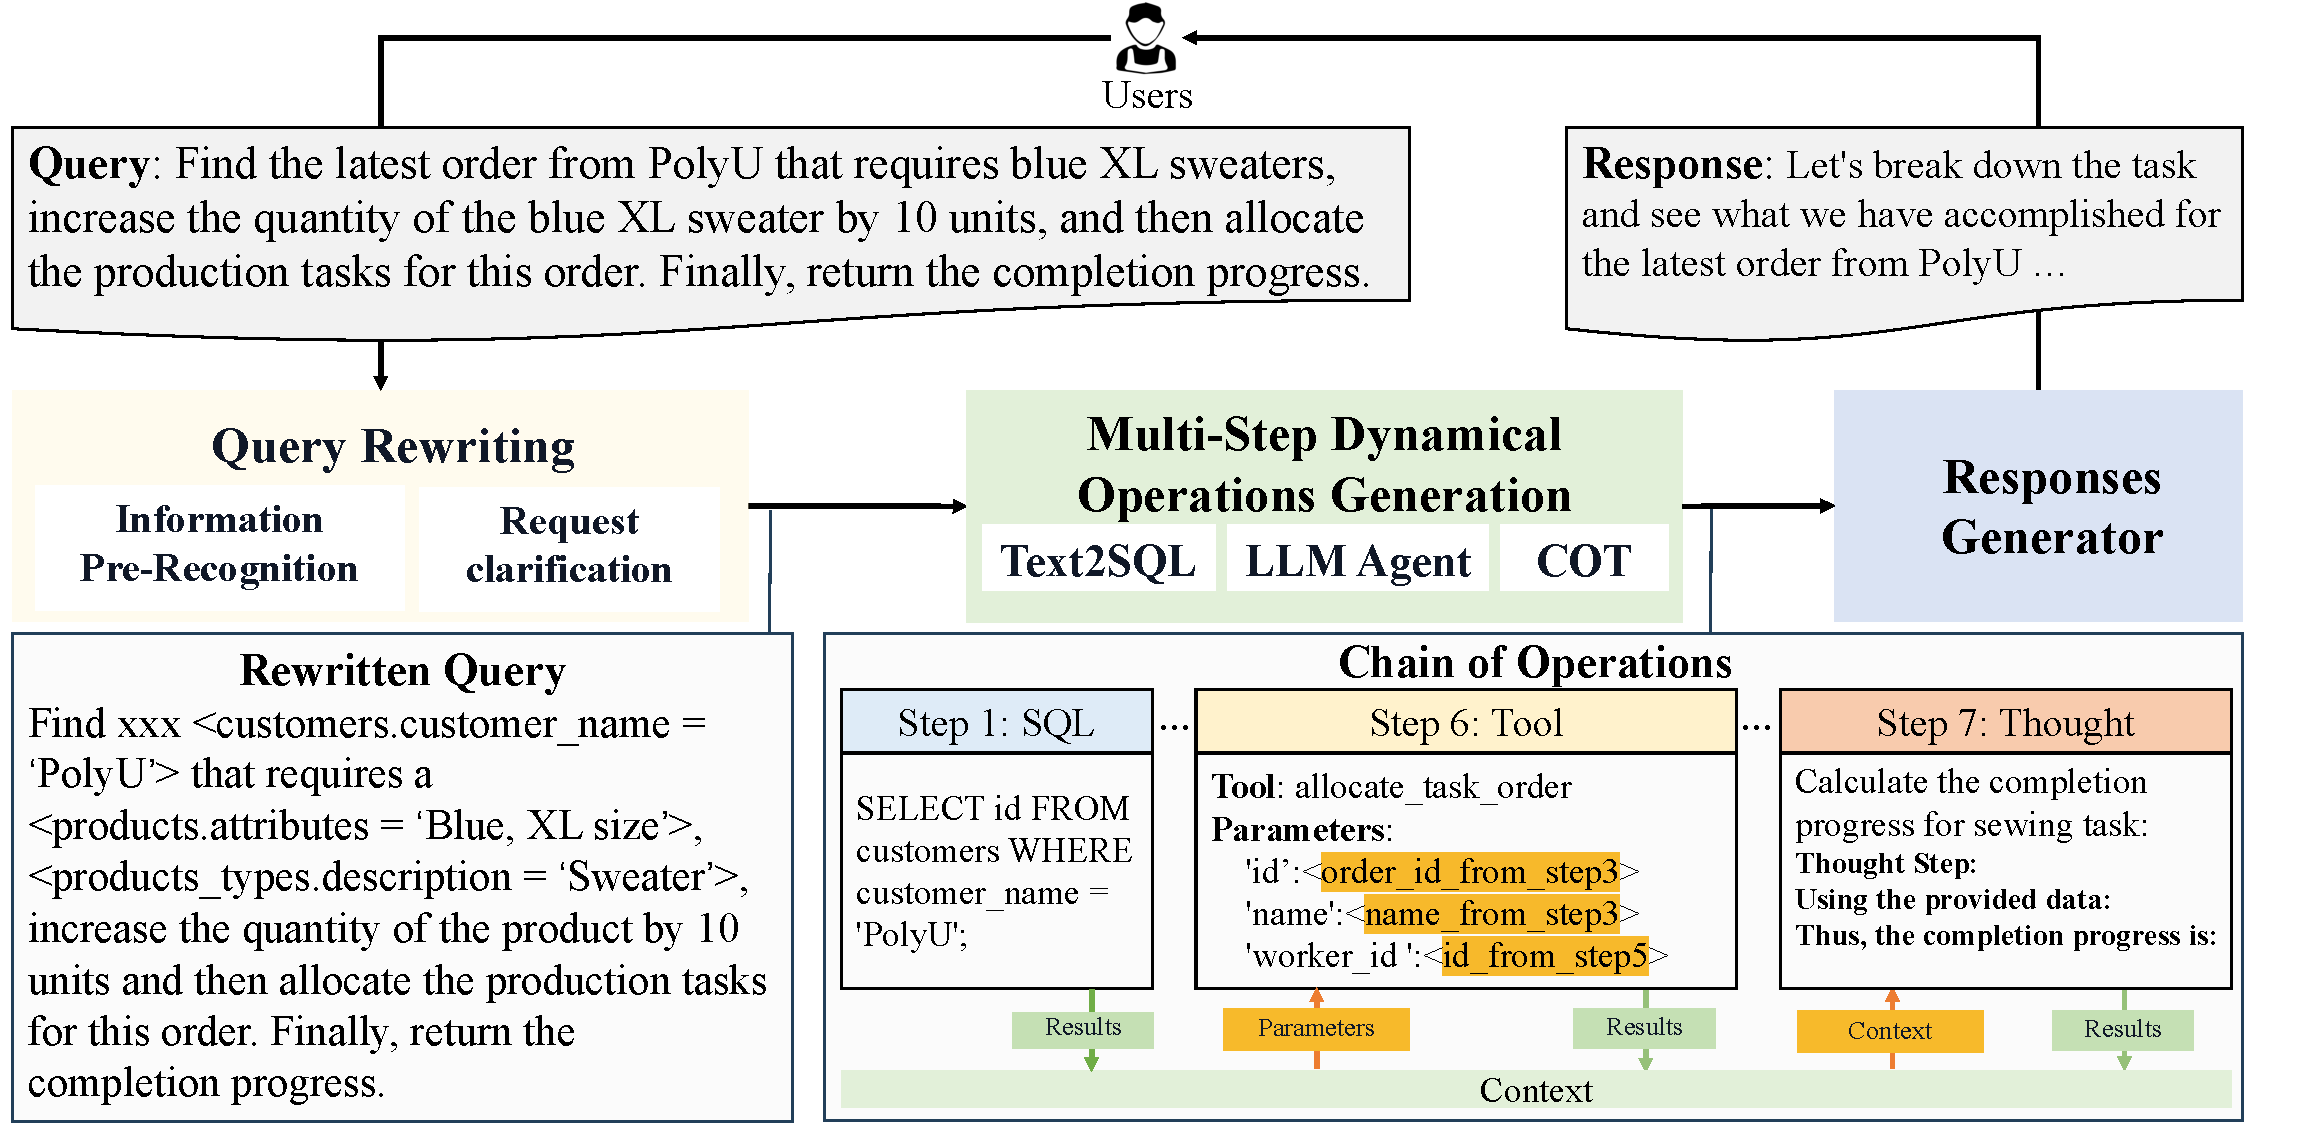
\includegraphics[width=1.05\linewidth]{figs/flow.pdf}
%% Use \caption command for figure caption and label.
\caption{Technical Framework of CWM}
\label{fig:cwm_framework}
%% https://en.wikibooks.org/wiki/LaTeX/Importing_Graphics#Importing_external_graphics
\end{figure}
The overall framework of CWM is illustrated in Figure~\ref{fig:cwm_framework}.
Upon receiving a textual request from the user, the CWM undergoes three stages, Request Rewriting, Multi-Step Dynamical Operations Generation, and Responses Generation.
To eliminate ambiguities from the user's original commands, the Request Re-writer uses an LLM to substitute entities in the request with precise descriptions that can be indexed in the database.
The Multi-step Dynamical Operations Generation develops a plan with step-by-step operations to handle the request and dynamically updates these operations.
The final stage, Responses Generation, summarizes the results from executing the operations and generates a textual response in markdown format for the user.
This section introduces the technical details of the Request Re-writer and Multi-step Dynamical Operations Generation processes.


\subsection{Request Re-writer for Preprocess}
When users interact with the CWM, they may input non-standardized or ambiguous information, which can introduce significant information bias in subsequent database operations.
% However, customers or workers are prone to providing non-standardized or ambiguous information to the CWM.
For example, both "PolyU" and "Hong Kong Polytechnic University" refer to the same entity associated with a record in the customer table.
If the real name stored in the database is "PolyU", once the user inputs "Hong Kong Polytechnic University" as the customer information, a generated SQL command may carry a wrong retrieve condition.
% The first step that the CWM shoub
Therefore, the first technical module of CWM is developed to
standardize the query for Entity disambiguation.

\begin{figure}
    \centering
    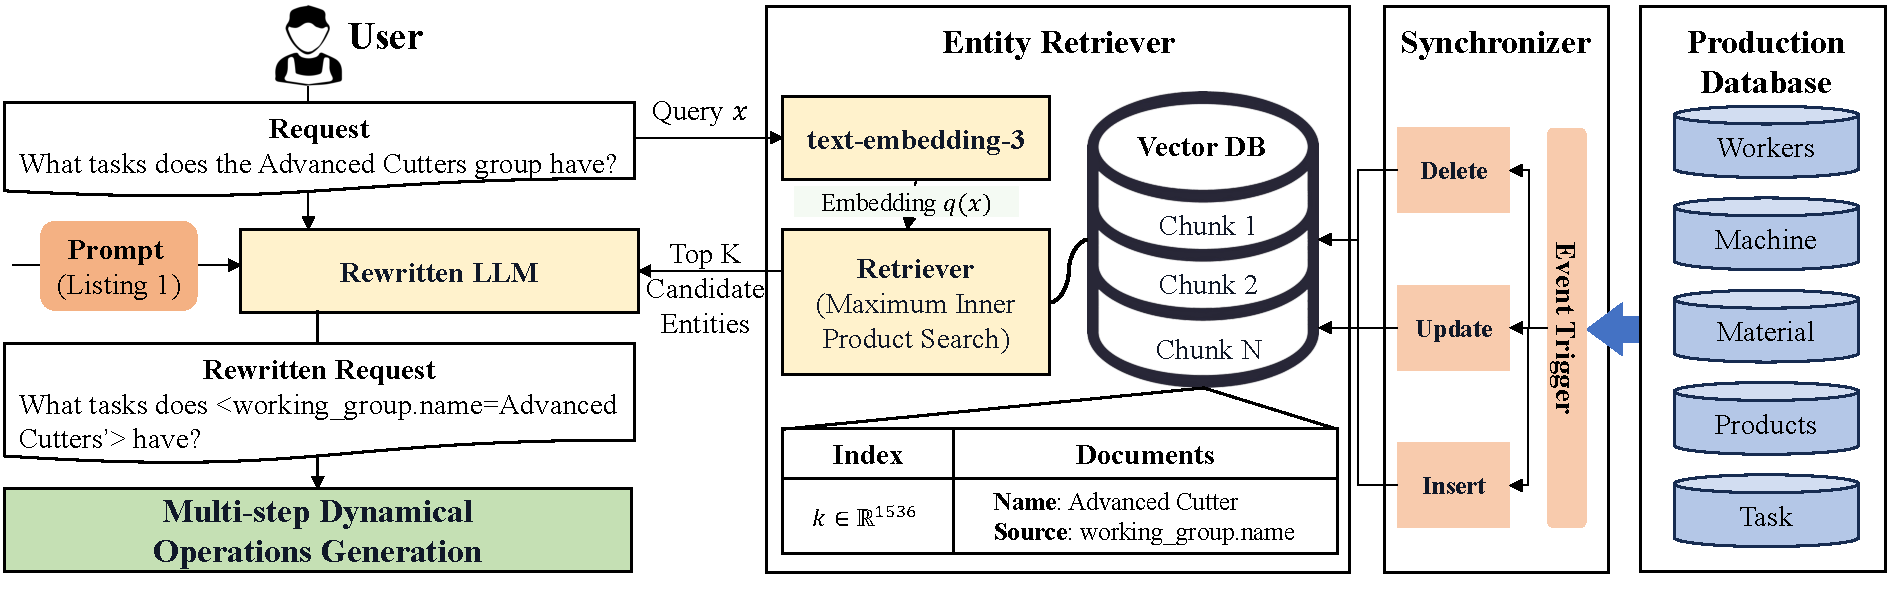
\includegraphics[width=\linewidth]{figs/query_rewrite.pdf}
    \caption{Workflow of Request Re-writer}
    \label{fig:tech_request_rewriter}
\end{figure}

The workflow of request re-writer is shown in Figure~\ref{fig:tech_request_rewriter}.
% The Entity Retriever dynamically maintains the embedding of registered entities from the production database in a vector database (DB).
The Entity Retriever is the core of the re-writer which dynamically maintains the embedding of registered entities from the production database in a vector DB.
Each entity is stored as a chunk comprising a key and the document.
The document consists of the entity's name appended to the database schema and column name.
The key represents the text embedding of the document generated by the OpenAI's text-embedding-3-large model.
A synchronizer is introduced to monitor database updates, triggering to insertion, updates, or deletions of the chunks in the vector DB.
For instance, if a customer modifies their name, it triggers a real-time update of the chunk associated with the customer's name.

After the user inputs the request $x$,
% In the first step, the complete user's request is input to the Entity Retriever for embedding.
The text-embedding-3-large model in the Entity Retriever is utilized to convert textual query into query vector $q(x)$. 
% By using Maximum Inner Product Search on the $q(x)$ and the keys of chunks, we search the Top-K similar chunks 
Subsequently, we identify the chunks with keys most similar to the query embedding $q(x)$ by employing the Top-K Maximum Inner Product Search.
% Finally, we employ the LLM's few-shot Named Entity Recognition capability to identify entities from the user's request~\cite{xie2023self} and retrieve the top-K relevant entities by a linguistic embedding module and a retriever.
Finally, we employ the LLM's zero-shot Named Entity Recognition capability to identify entities from the user's request~\cite{xie2023self} and use the retrieved chunks to rewrite the entity information with standardized format, {schema-field="information"} where the schema name, the field denotes the field name, and the "information" is the matched entity.
For example, the "Hong Kong Polytechnic University" will be transformed to \{customer.name="PolyU"\}.
The prompt for re-writing is shown in Listing~\ref{lst:query_rewrite}.
If the information provided by the user does not match any registered entity, it indicates that the user's query is not recognized, and the CWM will return to generate a question to the user for confirmation.

\begin{lstlisting}[style=prompt, label={lst:query_rewrite},caption={ Prompt for rewriting request},numberstyle=\scriptsize,aboveskip=0pt, belowskip=0pt]
(*@\color{red}{\# role}@*):
  You are a professional question optimization model. You can replace entity names in questions with standard entity names.

(*@\color{red}{\# Standard Entity Names}@*):
  The correspondence between entity names and possible standard entity names is as follows:
  {standard_entity_mapping}

(*@\color{red}{\# Output Requirements}@*):
  1. Convert entity names to the most probable standard entity names.
  2. Replace the original entity names with "<entity_type = standard_entity_name>"

(*@\color{red}{\# Output Examples}@*):
  1. Original Question:
  Orders of PolyU
  Rewritten Question:
  <customers.customer_name = 'PolyU'> orders
  2. Original Question:
  What are the sewing tasks that use silk
  Rewritten Question:
  What are the sewing tasks that use <products.product_name = 'Silk'>
  3. Original Question:
  What does the main warehouse have
  Rewritten Question:
  What does <warehouse.warehouse_name = 'Main Warehouse'> have
  4. Original Question:
  What tasks does the Advanced Sewers group have
  Rewritten Question:
  What tasks does <working_group.name = 'Advanced Sewers'> have

  {question}

(*@\color{red}{\# Rewritten Question}@*):
\end{lstlisting}

% Entity disambiguation by LLM
\subsection{Multi-step Dynamical Operations Planning and Execution}
% The foundation of CWM is transforming user's natural language queries into a series of basic operations.
In an MES, a request, such as assigning a task to a worker or placing an order for a customer, typically involves a series of complex operations.
To increase the controllability and reliability of CWM in handling complicated requests, this paper introduces \textbf{Multi-step Dynamical Operations Generation} to transform the natural language input from users to a series of executable basic operations in MES.
% This section will describe the details involved in generating and executing these operations.
Figure \ref{fig:tech_multi_step} illustrates the procedure for generating and executing multi-step dynamical operations.
\begin{figure}
    \centering
    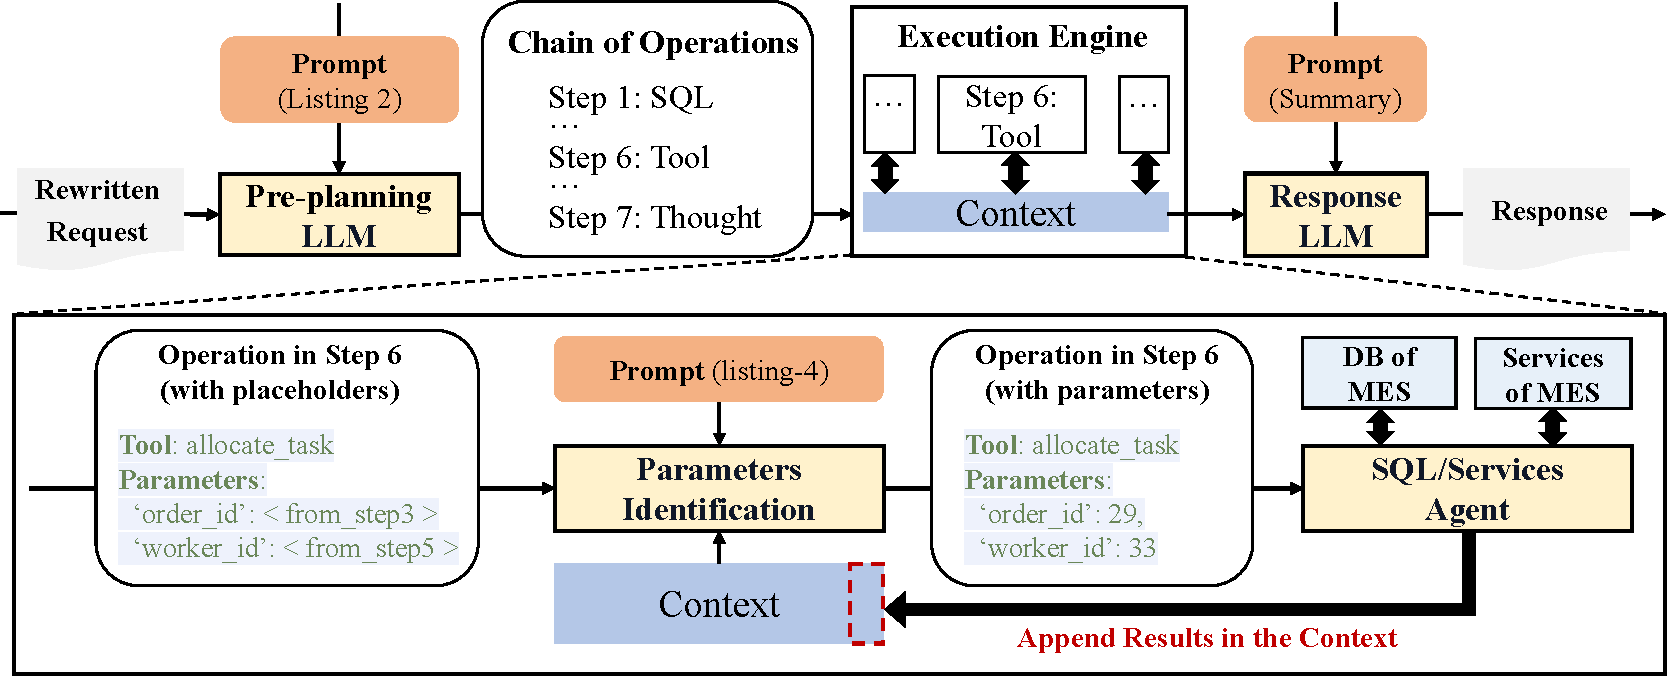
\includegraphics[width=\linewidth]{figs/multi_step.pdf}
    \caption{Multi-step Dynamical Operations Generation and Execution}
    \label{fig:tech_multi_step}
\end{figure}
This section begins with defining operations, followed by outlining pre-planning and execution processes. Subsequently, it delves into few-shot learning for integrating prior production guidelines, concluding with the final response generation.

\subsubsection{Definition of Operations}
% \subsubsectionfont{SQL}
% There are three kinds of operations in the the CWM.
A basic operation is either a request for invoking a tool, or executing a SQL command for operating the database, or a thought step.
As the most fundamental type of operation, 'SQL' represents accessing the MES database by generating an SQL command tailored to the specific purpose of the step.
The SQL commands are generated by the LLM, which is associated with Text2SQL, a significant and emerging research area in the application of LLMs.
% To enable the LLM to comprehend the logical relationships between entities and generate SQL commands in a correct sequence with proper grammar, 
% we export the textual database schemas and provide them as the system prompt to the Text2SQL LLM.

% Theoretically, if the Text2SQL module is intelligent enough, all requests in an MES can be resolved by directly manipulating the databases.
% However, an MES system always applies a set of production-related constraints on data editing.
% For example, assigning a production task to a worker is always associated with inserting a material allocation record in another table.
% As an illegal behavior, freely generating SQLs and arbitrarily changing the records in the databases are prohibited for MES.
% Therefore, an important issue for implementing CWM is restricting the behaviors of CWM to follow the pre-defined production logic and policies.

% The CWM addresses this issue from two perspectives, encapsulating tools and in-context learning.
% The details of in-context learning will be elaborated on in the next part.
As the second type of operation, the tools are associated with available API services provided by the MES and identified by the LLM agent according to four labels, \textbf{tool name, tool description, parameters, and parameter description}. 
We use LLM to autonomously decide which tool to invoke and determine the appropriate parameters based on the user's query or the retrieved results from the database.
In a MES, most tools comprise a series of data editing operations. 
Theoretically, if the Text2SQL module is intelligent enough, all requests excluding those that require external communication can be resolved by directly manipulating the databases.
However, an MES system always applies a set of production-related constraints on data editing.
For example, assigning a production task to a worker is always associated with inserting a material allocation record in another table.
As an illegal behavior, freely generating SQLs and arbitrarily changing the records in the databases are prohibited for MES.
Thus, it is essential to implement the tool operation as a means of encapsulating SQLs, ensuring that CWM actions adhere strictly to production protocols and policies.

The 'Thought' operation, the third category, complements the previous two by facilitating complex logic inference and mathematical calculations.
% The 'Thought' operation, the third category, enhances the previous two by enabling sophisticated logical deductions and mathematical computations. When
When the user's request involves summarization or statistical analysis, both 'Tool' and 'SQL' are only capable of retrieving relevant data.
Based on this, the 'Thought' step will generate a local CoT and infer the final result.
An example will be shown in the section \ref{sec:exp_cases}.

% The foundation of CWM is transforming user's natural language queries to a series of SQL commands for operating the database.
\begin{lstlisting}[style=prompt, label={lst:plan_prompt},caption={Prompt for generating the planned multi-step Operations},aboveskip=0pt, belowskip=0pt]
You are Chat With MES, a powerful AI assistant, a variant of ChatGPT that can 
1) decide to invoke some provided tools to solve the query. 
2) utilize the database of the Manufacturing Execution System as external symbolic memory. 
For any user query, you should always prioritize using the given tools to complete it.
The following are the tools you can use, including their names, descriptions, and input args.
"""
tool_allocate_task_order: Allocate the cutting task and sewing tasks for all products belonging to the order, and return
the allocated tasks and corresponding working groups.
{
    'order_id': {'title': 'Order Id', 'description': 'The order ID, an integer.', 'type': 'integer'}, 
    'order_name': {'title': 'Order Name', 'description': 'The order name, a string.', 'type': 'string'}
}

% Description of other Tools.
"""
Only if you cannot handle the command/query with any given tools, You are authorized to directly access the database.
In this case, you are an expert in databases, proficient in SQL statements and can use the database to help users. The details of tables in the database are delimited by triple quotes.
"""

-- Customer Table
CREATE TABLE `customers` (
  `id` VARCHAR(36) PRIMARY KEY COMMENT 'Customer ID',
  `customer_name` VARCHAR(255) NOT NULL COMMENT 'Customer Name'
);

% Other table creation scripts.

Please tell me what basic operations, including sql, tool,and thought, should I use in order to respond to the "USER INPUT". If it needs multiple operations, please list them step by step concisely, and indicate whether the operation involves calling a tool or  accessing a database via SQL. If there is no need to use any operations, reply to the "USER INPUT" directly.
At all times, you should prioritize using the provided tool. If the tool does not meet the requirements, only then may you resort to using SQL.
The output should be a markdown code snippet formatted in the following schema, including the leading and trailing "\`\`\`" and "\`\`\`":
```
Step1: <Description of first step>
SQL `SQL command for step1`

Step2: <Description of first step>
SQL `SQL command for step2`

Step3: <Description of second step>
Tool `Tool name, arguments for tool, purpose of using this tool`

Step4: <Description of fourth step>
Thought `Purpose of this intermediate reasoning step, what intermediate results are expected. and how to get them based on the results from the previous steps.`

```

Backticks are important and must be added at the beginning and end of the command for every step!

(*@\color{orange}{Here are some examples}@*):

USER INPUT: Retrieve all orders and item details for the Customer PolyU
ANSWER:
```
Step1: Retrieve the customer ID for the customer with the name "PolyU"

Execute:
SQL `SELECT id FROM customers WHERE customer_name = 'PolyU';`

Step2: Retrieve the details of products for each order, including product attributes and type description
Tool `tool_find_order_details, {'order_id': <order_id>}, Find the product details of an order`
```
% Omitted other few-shot examples.

(*@\color{blue}{USER INPUT}@*): Find the latest order from <customers.customer\_name = 'PolyU'> that requires a <products.attributes = 'Blue, XL size'> <products\_types.description = 'Sweater'>, increase the quantity of the <products.attributes = 'Blue, XL size'> <products\_types.description = 'Sweater'> by 10 units, and then automatically allocate the production tasks for this order.

(*@\color{blue}{ANSWER}@*): 

\end{lstlisting}

\subsubsection{Pre-planning operations}
% In Dynamic Multi-step Operations Planning, the CWM will strategize operations prior to execution, based
In Multi-step Dynamical Operations Planning and Execution, the CWM will pre-plan the operations prior to execution, 
Based on the prompt template from ChatDB~\cite{hu2023chatdb}, we design the prompt for generating multi-step  operations.
As shown in the prompt Listing~\ref{lst:plan_prompt}, it establishes the context and objectives for the LLM, including the instructions to the LLM, the details on the database schema and available tools, the output formats.
Certain redundant details are excluded, highlighted in red font.
% As demonstrated in prompt~\ref{lst:user_prompt}, the user prompt contains the original user query and specifies the output formats.
The content following USER INPUT represents the output from the query re-writer module.

In addition to the data schema and the description of available tools, CWM needs to understand the production guidelines, such as the order of accessing databases, the format of the data inserted into the table and some definitions and abbreviations in the garment industry.
Because each garment factory has customized guidelines and the knowledge base needs to be maintained dynamically, 
this study employs the training-free few-shot learning~\cite{hu2023chatdb} to inject the specific knowledge in the model. 
% It aids the CWM in grasping the MES's operational logic and schema interactions. Limited
It aids the CWM in understanding the MES's operational guidelines and the relationships among schema.
A deep understanding of the database structure is crucial for CWM to generalize effectively in handling arbitrary user inquiries.
Few-shot learning is accomplished by presenting some representative examples as system prompts.
Each example includes the chain of operations, the correct tools to invoke, and the SQL commands required to resolve the request.
% Table illustrates an example of assigning a task to workers.
We introduce three few-short learning examples in total for covering the primary difficult and representative cases of the garment MES, 1) placing orders, 2) analyzing task completion progress, and 3) retrieving product details of an order.
% The CWM is a to be generalized to other transactions which involve the operations on the same schemas.


\begin{lstlisting}[style=prompt, label={lst:param_prompt},caption={Parameters Identification prompt},numberstyle=\scriptsize,aboveskip=0pt, belowskip=0pt]
You are now the following python function: 
# "Find useful information in the results of the previous operating statement, and replace <> with the corresponding information. "
"If the operation type is 'Tool' and the tool must be invoked multiple times with varying parameters, "
"please output a list of tool operations with distinct parameters."
        
def populate_operation_statement(operation_str: str, previous_operation_results: list[list[dict]]) -> list[str]:
Only respond with your `return` value. Do not include any other explanatory text in your response.",

(*@\color{blue}{\# Operation}@*)
INSERT INTO order_product (order_id, product_id, number) VALUES ('<order_id>', '<red_tshirt_product_id>', 50)

(*@\color{red}{\# Historical Context}@*)
\end{lstlisting}

\subsubsection{Operation execution and dynamical parameters retrieval}
After the initial chain of operations are generated, the CWM employs regex matching to extract the operations command and their types and execute each operation one by one. 
Apart from the first operation, subsequent operation commands might contain placeholders, such as "<customer\_id\_step1>", that must be determined based on the context.
Before executing each command, CWM identifies these placeholders and uses LLM with prompt \ref{lst:param_prompt} to retrieve the specific parameters from the conversion context to update the operation command.
Finally, the operations with parameters are executed by accessing the database and the services of MES.
As shown in Figure~\ref{fig:tech_multi_step}, the results from executing each operation are appended in a conversation context.

\subsection{Response Generation}
After executing all operations, the context which consists of all intermediate results produced from each operation, will be fed to the Responses Generator. 
According to the original request from the user, the LLM-based generator will produce the final textual responses.
The structured records will be automatically organized as tables with the markdown format to give a good reading experience.
% In most chat tools, this markdown-formatted content is automatically rendered and the user will have a good reading experience.



% The prompt adheres to the CO-STAR format, as demonstrated in xxx.
% \lstset{
%  columns=fixed,       
%  numbers=left,                                        % 在左侧显示行号
%  numberstyle=\scriptsize\color{gray},                       % 设定行号格式
%  frame=none,                                          % 不显示背景边框
%  backgroundcolor=\color[RGB]{245,245,244},            % 设定背景颜色
%  keywordstyle=\color[RGB]{40,40,255},                 % 设定关键字颜色
%  numberstyle=\footnotesize\color{darkgray},           
%  commentstyle=\it\color[RGB]{0,96,96},                % 设置代码注释的格式
%  stringstyle=\rmfamily\slshape\color[RGB]{128,0,0},   % 设置字符串格式
%  showstringspaces=false,                              % 不显示字符串中的空格
%  language=text,                                        % 设置语言
% }




\section{Experiment}
\label{sec:exp}
% This section provides an in-depth introduction to the experimental design and results. 
Different types of users have diverse business requirements when utilizing MES, such as creating or querying orders, managing production tasks and material allocation, or handling inventory management. 
In the experimental section of this paper, we employ the garment manufacturing as the case scenario. 
Based on an existing, well-established garment MES platform, we simulate the operational processes of a clothing factory and generate simulated raw manufacturing system data. 
Building upon this experimental platform and dataset, we simulate common requests when users utilize an MES and investigate whether CWM can effectively comprehend and process various typical business requests described in natural language in the absence of a graphical user interface (GUI). 
% With limited external services and the permissions of accessing database, we explore the behaviors and the accuracy that CWM operates on the MES system and database to address users' requests and.
With restricted external service access and database permissions, we examine CWM's behavior and accuracy in operating within the MES system and database to fulfill user requests.

The experiment results demonstrate that CWM performs a high execution accuracy, 80\%, significantly outperforming Text2SQL baseline models. 
Multi-step operations planning and execution significantly contributes to a high execution success rate.
% ChatDB significantly outperforms the baseline model ChatGPT, highlighting the advantages of symbolic memory integration.
\subsection{Experimental Setup}

% \subsubsection{Settings of CWM}
% % 

\subsubsection{Simulated MES}
% To adapt to the use case of CWM and enable quantitative comparisons with other baselines, 
% we built a simple simulated garment MES by referencing a similar product in Huawei Cloud
To accommodate the utilization scenarios of CWM and facilitate quantitative comparisons with benchmarks, we developed a simulated garment MES by drawing upon a comparable product available in Huawei Cloud
~\footnote{\href{https://marketplace.huaweicloud.com/contents/da115457-cf31-47e1-bcff-965e5469d360\#productid=00301-608119-0--0}{YiZhi MES garment intelligent production management platform in HUAWEI CLOUD}}.
The constructed MES system incorporates the fundamental management components typical of garment manufacturing facilities, encompassing orders, customers, workers, materials, cutting operations, and sewing operations. 
The database in this simulated MES is a relational database involving 16 tables.
Their relations and foreign keys are shown in the ER diagram \ref{fig:er_diagram}.
We use the GPT-4 to generate the simulated data in the database, resulting in a total of 312 records.
\begin{figure}
        \centering
        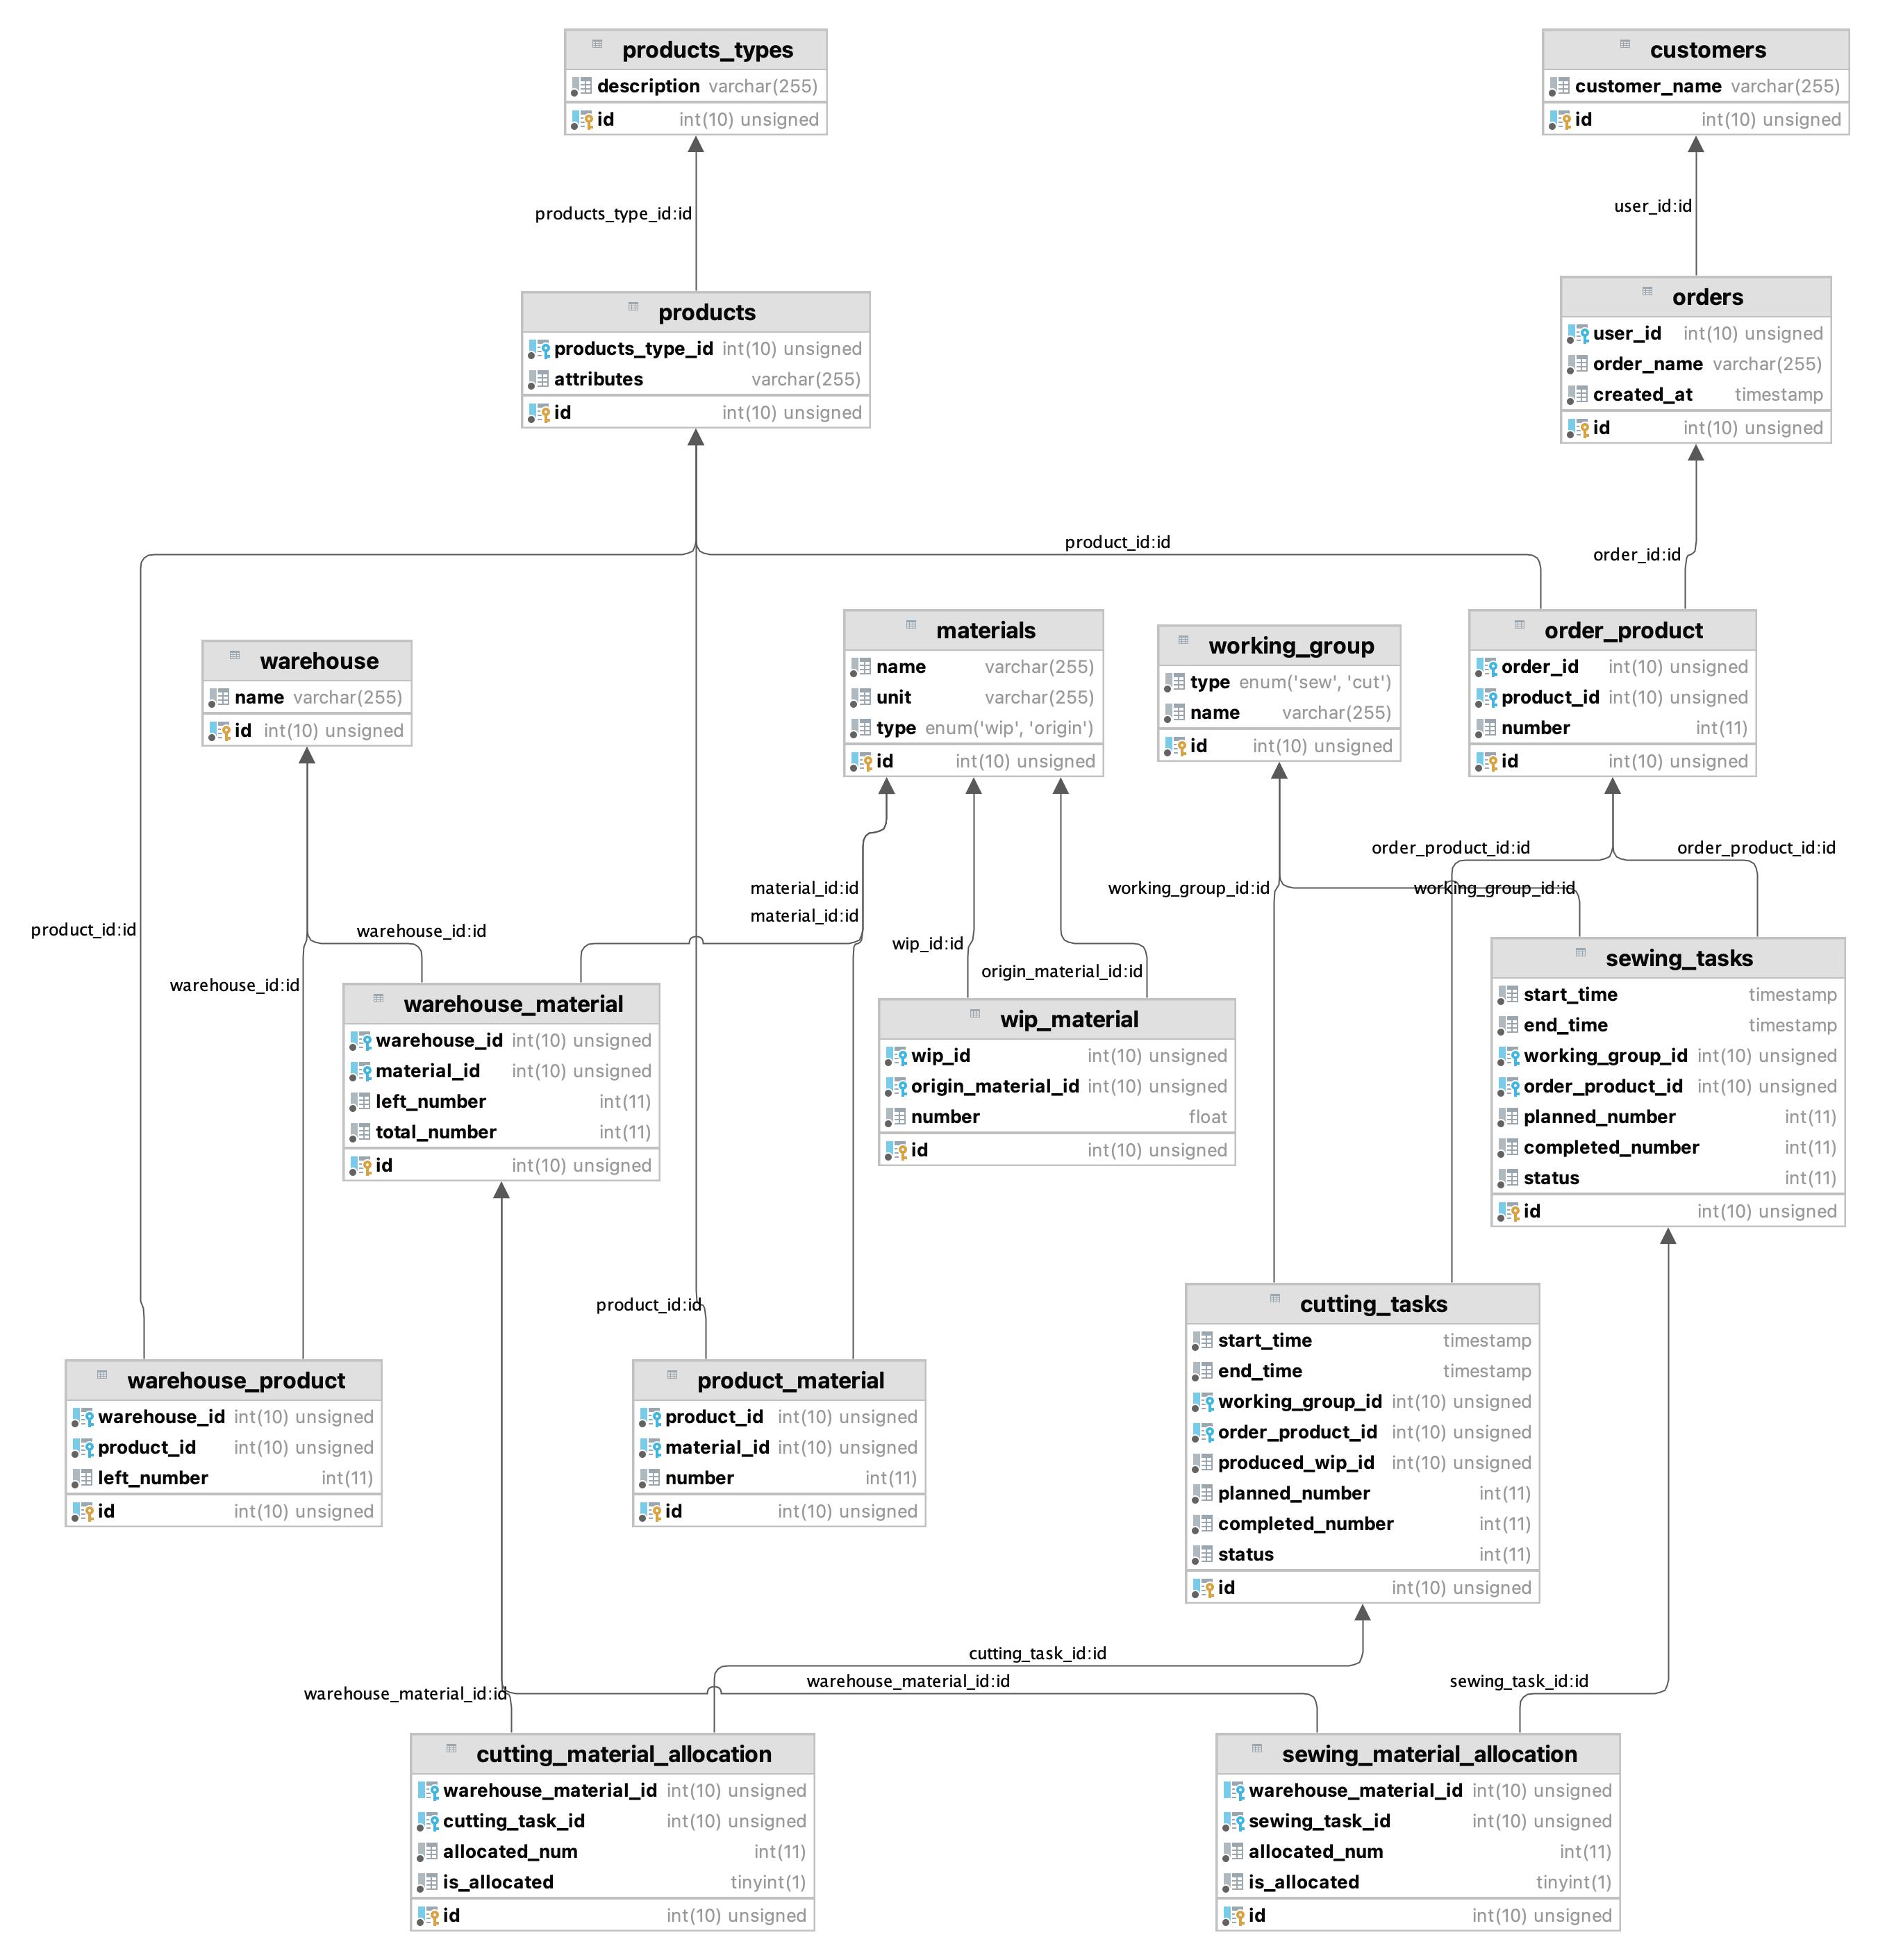
\includegraphics[width=1.1\linewidth]{figs/garment.png}
        \caption{ER Diagram}
        \label{fig:er_diagram}
\end{figure}
    
% Regarding the available tools that can be invoked in Multi-step Dynamic Operations Planning and Execution, table~\ref{tab:tools} enumerates the tools accessible to the LLM Agent. 
Table~\ref{tab:tools} enumerates the tools accessible to the LLM Agent. 
Given that the MES serves as a simulated platform for demonstration purposes, only four fundamental tools are presented to maintain simplicity.
\begin{table}[t]
\caption{Available tools in the simulated garment MES}
\label{tab:tools}
\resizebox{\textwidth}{!}{
\begin{tabular}{c|l|l}
\textbf{Tool} &
  \multicolumn{1}{|c|}{\textbf{Description}} &
  \multicolumn{1}{c}{\textbf{Parameters}} \\
  \hline
find\_order\_details &\makecell[l]{
  Find the product details of an order by the order ID.} &
  \textbf{order\_id}: ID of order\\ \hline
allocate\_task &
  Automatically allocate product order tasks to workers &
  \begin{tabular}[c]{@{}l@{}}\textbf{order\_id}: ID of order\\ \textbf{order\_name}: name of order\end{tabular} \\
  \hline
store\_materials &
  Automatically store materials in a free inventory. &
  \begin{tabular}[c]{@{}l@{}}\textbf{material\_id}: ID of material\\ \textbf{number}: number of stored materials\end{tabular} \\
  \hline
get\_busy\_workers &
  Find all working groups and their task counts. &
  None \\
  \hline
complete\_task &\makecell[l]{
  workers reporting the completion of specific production \\ tasks, it automatically adjusts the quantities of finished\\ products in the warehouse.} &
  \begin{tabular}[c]{@{}l@{}}\textbf{task\_id}: ID of task\\ \textbf{task\_type}: sewing or cutting\\ \makecell[l]{\textbf{quantity}: number of completed  \\ products or work-in-progress}\end{tabular} \\
\end{tabular}
}
\end{table}
% tool_get_busy_workers

\subsubsection{Requests Dataset}
Based on the database schema of the MES and the rows inside, we designed a requests dataset including 55 requests covering common operations in a garment factory: placing orders, checking inventory, work assignment, materials allocation, and so on.
We use the term 'request' instead of 'question' because it involves many commands rather than simply posing a question.
In actual production settings, requests may be initiated by two categories of users, workers and managers. Figure~\ref{fig:req_source} illustrates the distribution of the identities among 55 requests.
As the production manager is responsible for coordinating production tasks, workers, and resources, he is the primary user of CWM.
% Customer requests primarily involve placing orders and checking the progress of production.
Workers use this system to confirm allocated tasks and report their working progress.

Theoretically, all requests can be addressed using basic database operations--Inserting (I), Updating (U), and Querying (Q) and their combination to adjust the records in the database.
Figure \ref{fig:ques_types} presents the distribution of the required command types involved in all requests.
Most requests are data retrieval tasks which are slightly easier than the tasks requiring Inserting and Updating operations.
Figure~\ref{fig:complexity} evaluates the complexity distribution of requests as determined by the number of database tables involved in each request.
The most complex request requires the CWM to access five tables to complete it.
Approximately ten requests can be easily resolved by accessing only one table.


\begin{figure*}
\centering
  \begin{subfigure}{0.28\textwidth}
    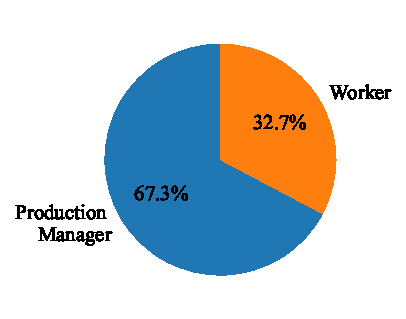
\includegraphics[width=\linewidth]{figs/questions_sources_user.pdf}
    \caption{Questioners.}
    \label{fig:req_source}
  \end{subfigure}
    \begin{subfigure}{0.32\textwidth}
    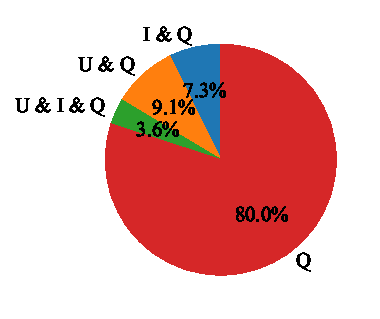
\includegraphics[width=\linewidth]{figs/questions_operation_type.pdf}
    \caption{Question types.}
    \label{fig:ques_types}
  \end{subfigure}
  \begin{subfigure}{0.3\textwidth}
    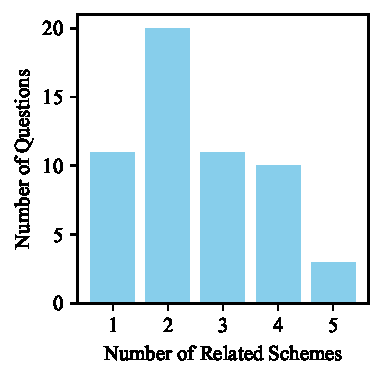
\includegraphics[width=\linewidth]{figs/questions_scheme_num.pdf}
    \caption{Complexity.}
    \label{fig:complexity}
  \end{subfigure}
  \caption{The distribution of request from the perspective of the operation types, identity, and complexity. The complexity is represented by the number of tables that need to be accessed to handle this question.}
\end{figure*}

\subsubsection{Evaluation}

We use the execution accuracy across all requests as the primary evaluation metric.
The response given by CWM for a request is regarded as correct when it meets two conditions: 
1) The CWM must adhere to the business logic of the MES and query or update the records in specific tables using either tools or pure SQL commands. 
2) It must consolidate the intermediate results from these operations and deliver a coherent response to the user's request.


The ground truth for requests is developed through semi-automatically process.
Initially, we use the CWM to produce both results and intermediate operation steps.
These outputs are then manually examined for potential inaccuracies.
In instances where errors are identified, additional prompts are consistently provided to the CWM to ensure that it yields the correct responses.
% e consistently provide sufficient hints to the CWM by supplying additional prompts until it produces the correct answers.

% The ground truth for requests is developed through a semi-automated process. Initially, the CWM is utilized to produce both results and intermediate operational steps. These outputs are then manually examined for potential inaccuracies. In instances where errors are identified, additional prompts are consistently provided to the CWM to ensure that it yields the correct responses.

During the evaluation of the CWM and other baselines, we introduce an auxiliary GPT-4o as an adjudicator, determining whether the generated chain of operations, operations commands, and responses closely approximate the ground truth.
For incorrect answers, the judge model is responsible for identifying the category and cause of the error. 
By analyzing the response processes of large models, we identified four types of errors:
\begin{itemize}
    \item \textbf{Information Deviation}: The LLM fails to identify the correct entity information from the user's input. For instance, while the user's request includes the customer name 'PolyU', the officially registered name in the database is 'Hong Kong Polytechnic University'.
    \item \textbf{Wrong CoT}: The LLM either fails to comprehend the user's intention or constructs an incorrect logical chain to address the problem.
    \item \textbf{Wrong Syntax}: There are syntax errors in the generated SQL commands and tool invocation statements.
    \item \textbf{Else}: Other errors that do not fit into the specified categories, such as errors in Mathematical Calculation. 
    % \item \textbf{Wrong Calculation}: The model errs in calculations, such as applying incorrect formulas or extracting incorrect parameters from the context.
\end{itemize}

The four types of errors have a "short-circuit" relationship.
If the model makes the "Information Deviation" error, any occurrences of "Wrong Syntax" and "Wrong CoT" in its response will not be counted.
Beyond evaluating Execution Accuracy and identifying individual errors within each category, we also measure token usage for responding to all requests, as this metric is relevant to cost and significant in practical applications.

\subsubsection{Details of implementing CWM}
All the LLMs used in CWM, including the query rewriting module, multi-step operations planner, and response generator, are based on GPT-4o by default, with their temperatures set to 0 to reduce the stochasticity during generation.
In section \ref{sec:ablation}, ablation studies were conducted to evaluate the selection of the foundational LLM. 
The agent responsible for the coordination of the provided tools is implemented utilizing the LangChain framework. 
% The foundational functions, which encompass chatting, summarizing, and generating multi-step operations, are developed using the OpenAI library.
We use Dify~\footnote{\href{https://github.com/langgenius/dify}{dify.ai}} to construct the graphical chatting window.
% The graphical chatting window is implemented by Dify~\footnote{\href{https://github.com/langgenius/dify}{dify.ai}}.
The source code of CWM, along with the simulated MES and benchmark requests, is publicly accessible in ~\footnote{\href{https://github.com/y18810919727/CWM}{https://github.com/y18810919727/CWM}}.
A test website is provided for convenient access and experience~\footnote{\href{https://dify.ai-fashion.cn/chat/muYb1xmFOw50PPWM}{Test website of the CWM}}.






% All the Large Language Models (LLMs) used in the CWM, including the query rewriting module, operations sequence generator, and response generator, are based on GPT-4o, with their temperatures set to 0 to minimize stochasticity during generation. The LLM agent responsible for coordinating the tools in the MES is implemented using the LangChain framework. The basic functions for textual chatting, summarizing, and generating multi-step operations are developed with the OpenAI library.
% To give a quantitative eva
\subsection{Two cases presenting how CWM handles user's requests}
\label{sec:exp_cases}
\begin{center}
\begin{longtable}{p{390pt}}
\caption{Example of querying the material usage}
    \label{tab:case_query_material}\\
    % \centering
    % \begin{tabular}{p{390pt}}
    \toprule
      \textbf{Question:}     \\
       % \makecell[l]{I am from The Hong Kong Polytechnic University. Today is July 2, 2024. Please \\ help me create an order for 50 red T-shirts in size M and 30 blue sweaters in size XL.} \\
       List the raw materials and quantities used for orders in June 2024? And organize it into the form of {raw materials: used quantity}.\\
          \hline
          % \textbf{Solution:}\\
          \textbf{Query Rewriting: }
          List the raw materials and quantities used for orders in June 2024? And organize it into the form of \{raw materials: used quantity\}.\\
 \hline
\textbf{Chain of Operations:}\\

\begin{lstlisting}[style=my_operation, label={lst:chain_of_operation}]
Step 1: Retrieve the order IDs for orders created in June 2024
SQL `SELECT id FROM orders WHERE created_at BETWEEN '2024-06-01' AND '2024-06-30';`

Step 2: Retrieve the product IDs and quantities for each order from June 2024
SQL `SELECT order_id, product_id, number FROM order_product WHERE order_id IN (<order_ids>);`

Step 3: Retrieve the work-in-progress (WIP) material IDs and quantities required for each product
Tool `tool_get_wip_materials, {'product_id': <product_id>}, Get the required work-in-progress materials for a product`

Step 4: Retrieve the original material IDs and quantities required for each WIP material
Tool `tool_get_original_materials, {'wip_id': <wip_id>}, Get the original materials for a work-in-progress material`

Step 5: Calculate the total quantity of each raw material used by multiplying the product quantity, WIP material quantity, and original material quantity
Thought `For each product, multiply the number of products by the quantity of each WIP material required, and then multiply by the quantity of each original material required for the WIP material. Sum these values for each raw material to get the total used quantity.`

Step 6: Organize the results into the form of {raw materials: used quantity}
Thought `Compile the calculated quantities from Step 5 into a dictionary format where keys are raw material names and values are the total used quantities.`
\end{lstlisting}\\ \hline

\hline
\textbf{Execution:}\\
\textbf{Step 1:} SQL, Retrieve the order IDs for orders created in June 2024.\\
Execute:\\
\lstinline!SELECT id FROM orders WHERE created_at BETWEEN '2024-06-01' AND '2024-06-30';! \\
\begin{lstlisting}[style=sql_command]
Database response:
+----+
| id |
+----+
| 10 |
| 11 |
| 12 |
+----+
\end{lstlisting}\\ \hline
\textbf{Step 2:} SQL, Retrieve the product IDs and product numbers for the orders found in Step 1.\\
Execute:\\
\lstinline!SELECT product_id, number FROM order_product WHERE order_id IN (10, 11, 12);! \\
\begin{lstlisting}[style=sql_command]
Database response:
+----------+------------+--------+
| order_id | product_id | number |
+----------+------------+--------+
|    10    |     30     |  150   |
|    11    |     20     |  120   |
|    12    |     7      |  330   |
+----------+------------+--------+
\end{lstlisting}\\ \hline
\textbf{Step 3:} Tool, Retrieve the work-in-progress (WIP) material IDs and quantities for the products found in Step 2\\
Execute:\\
\lstinline!'tool_get_wip_materials, {'product_id': 30}'!\\
\lstinline!'tool_get_wip_materials, {'product_id': 20}'!\\
\lstinline!'tool_get_wip_materials, {'product_id': 7}'!\\

\begin{lstlisting}[style=sql_command]
Results from invoking the tools:
Here are the work-in-progress (WIP) material IDs and quantities required for each product:
Product ID 30: {'Material ID': 2, 'Quantity': 5}, {'Material ID': 10, 'Quantity': 1}
Product ID 20: {'Material ID': 2, 'Quantity': 3}, {'Material ID': 6, 'Quantity': 4}
Product ID 7:  {'Material ID': 12,'Quantity': 5}, {'Material ID': 6, 'Quantity': 2}
\end{lstlisting}\\ \hline
\textbf{Step 4:} Tool, Retrieve the original material IDs and quantities required for each WIP material.\\
Execute:\\
\lstinline!tool_get_original_materials, {'wip_id': 2}! \\
\lstinline!tool_get_original_materials, {'wip_id': 10}! \\
\lstinline!tool_get_original_materials, {'wip_id': 6}! \\
\lstinline!tool_get_original_materials, {'wip_id': 12}!\\

\begin{lstlisting}[style=sql_command]
Results from invoking the tools:
WIP Material ID 2: {'Original Material ID': 1, 'Quantity': 0.4}, {'Original Material ID': 11, 'Quantity': 0.65}, {'Original Material ID': 3, 'Quantity': 0.2}
WIP Material ID 10: {'Original Material ID': 9, 'Quantity': 0.6}, {'Original Material ID': 1, 'Quantity': 0.35}, {'Original Material ID': 13, 'Quantity': 0.8}
WIP Material ID 6: {'Original Material ID': 5, 'Quantity': 0.75}, {'Original Material ID': 1, 'Quantity': 0.4}
WIP Material ID 12: {'Original Material ID': 11, 'Quantity': 0.7}, {'Original Material ID': 1, 'Quantity': 0.5}
\end{lstlisting}\\ \hline
\textbf{Step 5:} Thought, Calculate the total quantity of each raw material used by multiplying the product quantity, WIP material quantity, and original material quantity.\\
Output:\\
\begin{lstlisting}[style=sql_command]
To achieve the objective, we need to calculate the total quantity of each original material used based on the orders, products, WIP materials, and original materials. Here's a step-by-step breakdown:
1. **Retrieve Order Details:**
   - Orders in June 2024: IDs 10, 11, 12.
   - Order 10: Product ID 30, Quantity 150.
   ...
   
2. **WIP Materials Required for Each Product:**
   - Product ID 30:
     - WIP Material ID 2, Quantity 5.
     - WIP Material ID 10, Quantity 1.
   - Product ID 20:
   ...
   
3. **Original Materials Required for Each WIP Material:**
   - WIP Material ID 2:
     - Original Material ID 1, Quantity 0.4.
   ...
     
4. **Calculate Total Original Materials Used:**
   - **Product ID 30 (150 units):**
     - WIP Material ID 2: 150 * 5 = 750 units
       - Original Material ID 1: 750 * 0.4 = 300
   ...
   
5. **Sum the Quantities for Each Original Material:**

   - Original Material ID 1: 300 + 52.5 + 144 + 192 + 825 + 264 = 1777.5
   - Original Material ID 11: 487.5 + 234 + 1155 = 1876.5
   ...

These are the total quantities of each original material used based on the given orders and material requirements.
\end{lstlisting}\\ \hline
\textbf{Step 6:} Thought, Organize the results into the form of {raw materials: used quantity}.\\
Output:\\
\begin{lstlisting}[style=sql_command]
To compile the calculated quantities from Step 5 into a dictionary format, we will use the raw material names as keys and the total used quantities as values. Here is the dictionary:

```python
{
    "Original Material ID 1": 1777.5,
    "Original Material ID 11": 1876.5,
    "Original Material ID 3": 222,
    "Original Material ID 9": 90,
    "Original Material ID 13": 120,
    "Original Material ID 5": 855
}
```
\end{lstlisting}\\ \hline
% \textbf{Responses:}\\
% \hline
\end{longtable}
\end{center}

\begin{center}[t]
\begin{longtable}{p{390pt}}
\caption{Example of querying the material usage(without Multi-step Dynamical Operations Generation)}
    \label{tab:case_query_material_without_muti_step}\\
    \toprule
      \textbf{Question:}     \\
       % \makecell[l]{I am from The Hong Kong Polytechnic University. Today is July 2, 2024. Please \\ help me create an order for 50 red T-shirts in size M and 30 blue sweaters in size XL.} \\
       List the raw materials and quantities used for orders in June 2024? And organize it into the form of {raw materials: used quantity}.\\
          \hline
          % \textbf{Solution:}\\
          \textbf{Query Rewriting: }
          List the raw materials and quantities used for orders in June 2024? And organize it into the form of \{raw materials: used quantity\}.\\
 \hline

\hline
\textbf{Execution:}\\
SQL, To list the raw materials and quantities used for orders in June 2024, we need to find the orders created in June 2024, then join with order\_product to get the products, and finally join with product\_material to get the raw materials and their quantities.\\
Execute:\\
\lstinline!SELECT m.name AS raw_material, SUM(pm.number * @op.number@) AS used_quantity FROM orders o @JOIN order_product @ op ON o.id = op.order_id JOIN product_material pm ON op.product_id = pm.product_id JOIN materials m ON pm.material_id = m.id WHERE o.created_at BETWEEN '2024-06-01' AND '2024-06-30' AND @m.type = 'origin' @ GROUP BY m.name;! \\
% 目前发现这个SQL里有四个问题
% 第一个是JOIN product_material这里,根据多步操作里的逻辑,应该使用 wip_material 表来获取原材料的用量信息
% 第二个是op.number那里,材料用量是通过 cutting_tasks.completed_number 和 wip_material.number 计算得出的,op.number这玩意算的不知道是什么
% 第三个是m.type = 'origin'那里,多步生成里没这个条件,这里应该是大模型理解错误导致的
% 第四个是缺失了cutting_tasks 表的连接,cutting_tasks连接了订单产品和 WIP 材料,并提供了 completed_number,这是计算材料用量的重要依据
\begin{lstlisting}[style=sql_command]
Results from executing the SQL:
no results found.
\end{lstlisting}\\ \hline
\end{longtable}
\end{center}
Before presenting the quantitative evaluation results, this section provides two examples to demonstrate how CWM handles a user's request.
Table~\ref{tab:case_place_order} and \ref{tab:case_query_material_without_muti_step} compare CWM to the baseline GPT-4 using a sample request, by analyzing a sample request to query the raw materials consumed for orders in June 2024.
% The second example involves the task of querying and summarizing the inventory of materials within the warehouse, as illustrated in Table ~\ref{tab:case_query_material}. 
Given that the total material usage is calculated by aggregating the individual usage of each product within each order, a mathematical calculation is necessary to analyze the data retrieved from the previous steps. 
Compared to the previous example, the planned chain of operations includes two 'Thought' steps. 
During Step 5, the CWM utilizes the chain of thought (CoT) methodology to deconstruct this 'Thought' task further. 
This procedure is executed by GPT-4o without any prompts from the CWM. 
Step 6 effectively distills and arranges the retrieved results into the specified format.
Table~\ref{tab:case_query_material_without_muti_step} represents the results executed by the GPT-4o based Text2SQL model. 
The model generates a long SQL command containing three obvious errors marked with purple.
The errors result in no results being retrieved from the database.
The comparison clearly indicates decomposing complex tasks into sub-tasks can effectively reduce complexity, decrease the probability of model errors, and facilitate the incorporation of prior production guidelines into the LLM.


We specifically designed a highly challenging example to demonstrate CWM's capability in solving complex problem.
As shown in Table~\ref{tab:case_reorganize_production_plan}, the case involves rearranging the production plan because the expected delivery time of an order has been advanced.
The request involves third typical challenges.
First, the description of the order "dress order of Emily" is non-standardized reference, filled with ambiguity and vagueness.
In our simulated MES, the standardized order name is "Emily\_Dress".
CWM is required to identify the standardized entity names and formulate the appropriate retrieval SQL utilizing "Emily\_Dress". 
The second issue is the CWM must interpret the ambiguous reference, "the group with the minimum number of tasks".
The third challenge is CWM needs to understand the business guidelines of the factory, available tools (services), and the database schema, in order to autonomously plan a series of interdependent operations to process the request.

CWM decomposed this task into 20 steps, including 15 SQL operations, 2 Tool operations, and 3 Thought operations. 
Due to the large number of operations, the table omits specific execution logs and results, listing only the types and descriptions of the operations used. 
This example sufficiently demonstrates CWM's capability to replace the GUI in MES, as it can autonomously integrate external services and manipulate the database through natural language input, effectively handling complex requests in the manufacturing process.

% All questions  

% of fruit shop management records, referred to as the “Fruit Shop Dataset”. This dataset simulates four common operations in a shop: purchasing, selling, changing prices, and goods returns. We ensure that all historical records are valid and do not encounter issues such as negative inventory. We generate 70 records arranged in chronological order, totaling approximately 3.3k tokens, which is within the maximum token length limit of ChatGPT (4096 tokens).




\begin{center}
\begin{longtable}{p{390pt}}
\caption{Example of reorganize production plan}
    \label{tab:case_reorganize_production_plan}\\
    \toprule
      \textbf{Question:} \\
       The dress order of Emily requires delivery by April 5, 2024. Please re-arrange the production plan and assign tasks to the task group with the fewest tasks currently. Provide a new production plan.\\
          \hline
          \textbf{Query Rewriting: }
          The <orders.order\_name = 'Emily\_Dress'> order requires delivery by April 5, 2024. Please re-arrange the production plan and assign tasks to the task group with the fewest tasks currently. Provide a new production plan.\\
 \hline
\textbf{Chain of Operations:}\\

\begin{lstlisting}[style=my_operation, label={lst:chain_of_operation}]
Step 1: Retrieve the order ID for the order with the name "Emily_Dress"
SQL `SELECT id FROM orders WHERE order_name = 'Emily_Dress';`

Step2: Retrieve the product details related to the order\n["tool_find_order_details, {'order_id': 3}, Find the product details of an order"]
Tool `tool_find_order_details, {'order_id': 3}, Find the product details of an order`

Step3: Retrieve the current cutting task's working group ID for the order
SQL `SELECT working_group_id FROM cutting_tasks WHERE order_product_id IN (SELECT id FROM order_product WHERE order_id = 3);`

Step4: Retrieve the current sewing task's working group ID for the order
SQL `SELECT working_group_id FROM sewing_tasks WHERE order_product_id IN (SELECT id FROM order_product WHERE order_id = 3);`

Step5: Get the current list of all working groups and their task counts\ntool_get_busy_workers, {}, Get the current list of all working groups and their task counts
Tool `tool_get_busy_workers, {}, Get the current list of all working groups and their task counts`

Step6: Compare the task counts of all cutting groups obtained in Step5 and identify the group with the fewest tasks.
Thought `Compare the task counts of all cutting groups obtained in Step5 and identify the group with the fewest tasks.`

Step7: Compare the task counts of all sewing groups obtained in Step5 and identify the group with the fewest tasks.
Thought `Compare the task counts of all sewing groups obtained in Step5 and identify the group with the fewest tasks.`

Step8: Retrieve the produced WIP ID from the cutting tasks
SQL `SELECT produced_wip_id FROM cutting_tasks WHERE order_product_id IN (SELECT id FROM order_product WHERE order_id = 3);`

Step9: Update the status of the original cutting tasks to 0 (stopped)
SQL `UPDATE cutting_tasks SET status = 0 WHERE order_product_id IN (SELECT id FROM order_product WHERE order_id = 3);`

\end{lstlisting}\\
\begin{lstlisting}[style=my_operation, label={lst:chain_of_operation}]

Step10: Create new cutting tasks with the new working group ID and set the new deadline to April 5, 2024
SQL `INSERT INTO cutting_tasks (start_time, end_time, working_group_id, order_product_id, produced_wip_id, planned_number, status) VALUES (CURRENT_TIMESTAMP, '2024-04-05 23:59:59', 6, 21, 8, 140, 1);`

Step11: Create new cutting tasks with the new working group ID and set the new deadline to April 5, 2024
SQL `INSERT INTO cutting_tasks (start_time, end_time, working_group_id, order_product_id, produced_wip_id, planned_number, status) VALUES (CURRENT_TIMESTAMP, '2024-04-05 23:59:59', 6, 29, 10, 150, 1);`

Step12: Create new cutting tasks with the new working group ID and set the new deadline to April 5, 2024
SQL `INSERT INTO cutting_tasks (start_time, end_time, working_group_id, order_product_id, produced_wip_id, planned_number, status) VALUES (CURRENT_TIMESTAMP, '2024-04-05 23:59:59', 6, 13, 12, 130, 1);`

Step13: Create new cutting tasks with the new working group ID and set the new deadline to April 5, 2024
SQL `INSERT INTO cutting_tasks (start_time, end_time, working_group_id, order_product_id, produced_wip_id, planned_number, status) VALUES (CURRENT_TIMESTAMP, '2024-04-05 23:59:59', 6, 5, 6, 120, 1);`

Step14: Update the status of the original sewing tasks to 0 (stopped)
SQL `UPDATE sewing_tasks SET status = 0 WHERE order_product_id IN (SELECT id FROM order_product WHERE order_id = 3);`

Step15: Create new sewing tasks with the new working group ID and set the new deadline to April 5, 2024
SQL `INSERT INTO sewing_tasks (start_time, end_time, working_group_id, order_product_id, planned_number, status) VALUES (CURRENT_TIMESTAMP, '2024-04-05 23:59:59', 10, 21, 140, 1);`

Step16: Create new sewing tasks with the new working group ID and set the new deadline to April 5, 2024
SQL `INSERT INTO sewing_tasks (start_time, end_time, working_group_id, order_product_id, planned_number, status) VALUES (CURRENT_TIMESTAMP, '2024-04-05 23:59:59', 10, 29, 150, 1);`

Step17: Create new sewing tasks with the new working group ID and set the new deadline to April 5, 2024
SQL `INSERT INTO sewing_tasks (start_time, end_time, working_group_id, order_product_id, planned_number, status) VALUES (CURRENT_TIMESTAMP, '2024-04-05 23:59:59', 10, 13, 130, 1);`

Step18: Create new sewing tasks with the new working group ID and set the new deadline to April 5, 2024
SQL `INSERT INTO sewing_tasks (start_time, end_time, working_group_id, order_product_id, planned_number, status) VALUES (CURRENT_TIMESTAMP, '2024-04-05 23:59:59', 10, 5, 120, 1);`

\end{lstlisting}\\ 
\begin{lstlisting}[style=my_operation, label={lst:chain_of_operation}]
Step19: Check material inventory for required materials
SQL `SELECT pm.material_id, pm.number, wm.left_number FROM product_material pm JOIN warehouse_material wm ON pm.material_id = wm.material_id WHERE pm.product_id IN (SELECT product_id FROM order_product WHERE order_id = 3);`

Step20: Compile the new cutting and sewing group information, new task schedule, material inventory status, and expected completion date into a report.
Thought `Compile the new cutting and sewing group information, new task schedule, material inventory status, and expected completion date into a report.`
\end{lstlisting}\\ \hline
\end{longtable}
\end{center}









% The LLM first identifies the customer ID based on the customer name provided by the user.

% Please add the following required packages to your document preamble:
% \usepackage{multirow}
% \begin{table}[ht]
% \centering
% \begin{tabular}{c|c|c|ccc}
% \hline
% \multirow{2}{*}{Models} &
%   \multirow{2}{*}{\begin{tabular}[c]{@{}c@{}}Execution \\ Accuracy\end{tabular}} & \multirow{2}{*}{Tokens}&
%   \multicolumn{3}{c}{Causes of errors} \\
%  &
%    & &
%   \begin{tabular}[c]{@{}c@{}}Wrong \\ CoT\end{tabular} &
%   \begin{tabular}[c]{@{}c@{}}Wrong\\ SQL\end{tabular} &
%   \begin{tabular}[c]{@{}c@{}}Information\\ Deviation\end{tabular} \\ \hline
% GPT-3.5                                                      & 45.5\% &  111370 & 16 & 9 & 5  \\
% \hline
% GPT-4o                                                        & 58.2\% &  109646 & 6 & 13 & 4  \\
% \hline
% \begin{tabular}[c]{@{}c@{}}CWM\\ (w/o rewriter)\end{tabular} & 72.7\% &  455102 & 6 & 5 & 4 \\
% \hline
% \begin{tabular}[c]{@{}c@{}}CWM\\ (w/o Multiple-Step \\operations)\end{tabular} & 67.2\% &  152458 & 8 & 10 & 0 \\
% \hline
% \textbf{CWM}                                                          & \textbf{80\%} &  487928 & 4 & 4 & 0  \\
% \hline
%   % \multicolumn{1}{l|}{} &
%   \multicolumn{1}{l}{} &
%   \multicolumn{1}{l}{} &
%   \multicolumn{1}{l}{}
% \end{tabular}
% \end{table}


\subsection{Main results}

\begin{table}[ht]
\centering
\caption{Main results}
\label{tab:main_tab}
\resizebox{\textwidth}{!}{
\begin{tabular}{c|c|c|cccc}
\hline
\multirow{2}{*}{Models} &
  \multirow{2}{*}{\begin{tabular}[c]{@{}c@{}}Execution \\ Accuracy\end{tabular}} & \multirow{2}{*}{Tokens}&
  \multicolumn{4}{c}{Causes of errors} \\
   & & &
  % \begin{tabular}[c]{@{}c@{}}Wrong \\ CoT\end{tabular} &
  % \begin{tabular}[c]{@{}c@{}}Wrong\\ Syntax\end{tabular} &
  % \begin{tabular}[c]{@{}c@{}}Wrong\\ Calculation\end{tabular} &
  % \begin{tabular}[c]{@{}c@{}}Information\\ Deviation\end{tabular} \\ \hline
  \begin{tabular}[c]{@{}c@{}}Information\\ Deviation\end{tabular} &
  \begin{tabular}[c]{@{}c@{}}Wrong \\ CoT\end{tabular} &
  \begin{tabular}[c]{@{}c@{}}Wrong\\ Syntax\end{tabular} &
  \begin{tabular}[c]{@{}c@{}}Else\end{tabular} \\ \hline
GPT-3.5                                                      & 25.5\% &  319866 & 3 & 28 & 9 & 1 \\
\hline
GPT-4o                                                        & 60\% &  311176 & 3 & 14 & 0 & 5  \\
\hline
\begin{tabular}[c]{@{}c@{}}CWM\\ (w/o re-writer)\end{tabular} & 70.9\% &  439947 & 3 & 10 & 1 & 2 \\
\hline
\begin{tabular}[c]{@{}c@{}}CWM\\ (w/o Multiple-\\Step operations)\end{tabular} & 61.8\% & 401771 & 0 & 18 & 3 & 0 \\
\hline
\textbf{CWM}                                                          & \textbf{80\%} &  436057 & 0 & 7 & 1 & 3  \\
\hline
  % \multicolumn{1}{l|}{} &
  \multicolumn{1}{l}{} &
  \multicolumn{1}{l}{} &
  \multicolumn{1}{l}{}
\end{tabular}
}
\end{table}
This section illustrates the quantitative performance of the CWM in comparison to baseline models as shown in Table \ref{tab:main_tab}.% we compared the quantitative performance of CWM with several baselines.
As two weak baselines, the original GPT-3.5 and GPT-4.0 are utilized as text2SQL engines to generate a single SQL command for handling the user's request.
The execution accuracy of GPT-4o is 60\%, significantly lower than the solutions based on the CWM architecture. 
This indicates that workflow engineering is essential for enabling the foundational LLM to operate an MES effectively.
Unavoidably, the use of a complex workflow inevitably leads to increased token usage.
% , approximately four times greater than when employing a Large Language Model (LLM) alone.

Considering that the CWM is analogous to the integration of a Request re-writer and Multiple-step operations, we have undertaken an individual assessment of each component's contribution.
The Request re-writer can efficiently tackle the Information Deviation, contributing about 13\% accuracy improvement.
% The Multiple-step Dynamical Operations Generation is the most important part in CWM to reduce the errors and contributes about 18.3\% improvement.
% By breaking a complicated task into several basic steps, generating a SQL command for a single step is much easier and the wrong syntax is efficiently avoided.
The query re-writer effectively addresses Information Deviation, contributing approximately a 9\% increase in accuracy. 
The Multi-step Dynamic Operations Planning and Execution is the most crucial component of the CWM, reducing errors and providing an approximate 18.2\% improvement. 
% Decomposing a complex task into simpler constituent steps facilitates the generation of SQL commands for each respective step, significantly minimizing the likelihood of syntax errors. 
% Furthermore, 
Handling the request step-by-step ensures alignment with human intent and pre-existing knowledge within a specified context, thereby leading to a reduction in errors related to both the chain of thought (COT) and computational processes.

\begin{figure}[t]%% placement specifier
%% Use \includegraphics command to insert graphic files. Place graphics files in 
%% working directory.
\centering%% For centre alignment of image.
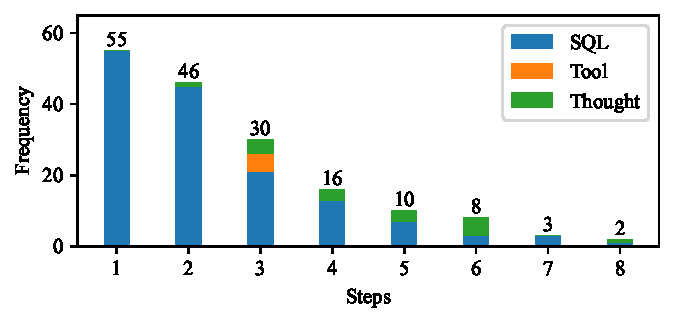
\includegraphics[width=0.8\linewidth]{figs/stacked_bar_chart.pdf}
%% Use \caption command for figure caption and label.
\caption{Frequency of each operation type invoked in each step.}
\label{fig:dist_operation}
%% https://en.wikibooks.org/wiki/LaTeX/Importing_Graphics#Importing_external_graphics
\end{figure}
Figure \ref{fig:dist_operation} shows the total times for executing three different kinds of operations at each step for 55 requests.
The process is limited to a maximum of 8 steps. 
Most requests, accounting for 45, can be resolved within 4 steps.
In the initial stages, SQL operations are predominant, as the CWM necessitates data retrieval from the database prior to engaging in subsequent data processing and tool invocation activities. 
The processes involving thought typically take place in the subsequent stages when requests require mathematical computation. 
The integration of these three types of operations is nearly sufficient to address all requests within the CWM.

\subsection{Ablation study}
\label{sec:ablation}
\begin{table}[ht]
\centering
\caption{Results in ablation study}
\label{tab:ablation}
\resizebox{0.85\textwidth}{!}{
\begin{tabular}{c|c|c|c|cccc}
\hline
\multirow{2}{*}{\centering \arraybackslash \begin{tabular}[c]{@{}c@{}}Foundation \\ Model\end{tabular}} &
\multirow{2}{*}{\centering \arraybackslash Thought} & 
\multirow{2}{*}{\centering \arraybackslash Tool} &
\multirow{2}{*}{\centering \arraybackslash \begin{tabular}[c]{@{}c@{}}Execution \\ Accuracy\end{tabular} }&
\multicolumn{3}{c}{Causes of errors} \\
 &
   & & &
  % \begin{tabular}[c]{@{}c@{}}Wrong \\ CoT\end{tabular} &
  % \begin{tabular}[c]{@{}c@{}}Wrong\\ Syntax\end{tabular} &
  % \begin{tabular}[c]{@{}c@{}}Wrong\\ Calculation\end{tabular} &
  % \begin{tabular}[c]{@{}c@{}}Information\\ Deviation\end{tabular}
  % \begin{tabular}[c]{@{}c@{}}Wrong\\ Understanding\end{tabular}
  % \begin{tabular}[c]{@{}c@{}}Information\\ Deviation\end{tabular} 
  % \\ \hline

  
  \begin{tabular}[c]{@{}c@{}}Wrong \\ CoT\end{tabular} &
  \begin{tabular}[c]{@{}c@{}}Wrong\\ Syntax\end{tabular} &
  \begin{tabular}[c]{@{}c@{}}Else\end{tabular} \\ \hline
  
GPT-4o     &  \checkmark & \checkmark  & 80\% & 7 & 1 & 3 \\ \hline
GPT-4o     &  \checkmark & $\times$  & 65\%   & 15 & 3 & 1 \\ \hline
GPT-4o     &  $\times$ & \checkmark  & 67\%   & 16 & 0  & 2 \\ \hline
GPT-3.5    & \checkmark & \checkmark  & 16\%  & 26 & 18& 2 \\ \hline
% ???     & \checkmark & \checkmark   &  &  &  &   \\ \hline
\end{tabular}
}
\end{table}

Within the Multi-step Dynamical Operation framework, the 'Tool' and 'Thought' operations are important in augmenting the precision of CWM's execution.
To measure the impact of each operation type, we performed extensive ablation studies to assess CWM performance when lacking one operation type.
The study further examines how the fundamental LLM in CWM affects performance. 

According to Table~\ref{tab:ablation}, excluding 'Thought' or 'Tool' operations significantly drops CWM execution accuracy. 
The presence of 'Tool' operations provides a marginally greater contribution compared to 'Thought'.% 'Thought' operations help lower calculation errors.
% Just like the example shown in Table \ref{tab:case_query_material} which demonstrates a meticulous approach to retrieve data and logically deducing the answer. 
Without thought processes, the model struggles with reasoning and calculations. 
As most dataset requests are straightforward, removing 'Thought' does not greatly impact performance.

As a greater role in the operations of CWM, the 'Tool' operations are important for handling the requests that require extensive prior knowledge of production, such as task allocation and material allocation.
Without the 'Tool', the CWM must generate a series of complex SQL commands to simulate the functions of the missing tools. 
In this process, commands with incorrect syntax may be produced, and the number of 'Wrong Syntax' will increase.

Finally, we replaced the foundational LLMs in the CWM with other advanced alternatives.
The results demonstrate that the intelligence of the foundation model significantly impacts the CWM's performance.
The CWM based on GPT-3.5 fails to generate syntactically correct SQL.
The accuracy is even lower than that of the GPT-3.5 without the CWM framework.
This suggests that as the cognitive abilities of large models develop and further align with human intentions, the capabilities of CWM can advance in parallel.

% Thought

% \subsection{Analysis of the generated operations}











% \begin{center}
% \begin{longtable}{p{390pt}}
% \caption{Example of creating an order}
%     \label{tab:case_place_order}\\
%     % \centering
%     % \begin{tabular}{p{390pt}}
%     \toprule
%       \textbf{Question:}     \\
%        % \makecell[l]{I am from The Hong Kong Polytechnic University. Today is July 2, 2024. Please \\ help me create an order for 50 red T-shirts in size M and 30 blue sweaters in size XL.} \\
%        What products are included in PolyU's January 2024 orders?\\
%           \hline
%           \textbf{Query Rewriting: }\\
%            What products are included in <customers.customer\_name = 'PolyU'>'s <orders.order\_name = 'Order for PolyU'>?\\
% \hline
% \end{longtable}
% \end{center}     



% \begin{lstlisting}
% Step1: Identify the customer ID for "The Hong Kong Polytechnic University".

% Execute:
% SELECT id FROM customers WHERE customer_name = 'PolyU';

% Results from executing the SQL:
% +----+
% | id |
% +----+
% | c1 |
% +----+


% Step2: Identify the product type IDs for "T-shirt" and "Sweater".

% Execute:
% SELECT id FROM products_types WHERE description IN ('T-shirt', 'Sweater');

% Results from executing the SQL:
% +-----+
% |  id |
% +-----+
% | pt1 |
% | pt7 |
% +-----+


% Step3: Identify the product IDs for "Red, M size T-shirt" and "Blue, XL size Sweater".

% Execute:
% SELECT id FROM products WHERE (products_type_id = 'pt1' AND attributes = 'Red, M size') OR (products_type_id = 'pt7' AND attributes = 'Blue, XL size');

% Results from executing the SQL:
% +-----+
% |  id |
% +-----+
% |  p1 |
% | p17 |
% +-----+


% Step4: Create a new order for the user.

% Execute:
% INSERT INTO orders (id, user_id, order_name) VALUES (UUID(), 'c1', 'Order for PolyU');

% Results from executing the SQL:
% insert data successfully.


% Step5: Establish the relationship between the order and products, and specify the quantities.

% Execute:
% INSERT INTO order_product (id, order_id, product_id, number) VALUES (UUID(), (SELECT id FROM orders WHERE user_id = 'c1' ORDER BY created_at DESC LIMIT 1), 'p1', 50), (UUID(), (SELECT id FROM orders WHERE user_id = 'c1' ORDER BY created_at DESC LIMIT 1), 'p17', 30);
% \end{lstlisting}

\section{Discussion}
\label{sec:discussion}

% LLM Workflow engineering reduces system complexity by breaking down a complex task into smaller steps, integrating more human supervision and control in generating responses. 
% It decreases reliance on prompting techniques and model reasoning capabilities, thereby enhancing the performance of LLM applications for complex tasks and improving observability, interpretability, stability, and fault tolerance.

% \begin{table}[ht]
%     \centering
%     \caption{Comparison between LLM applications in Serious and Creative Scenarios}
%     \begin{tabular}{c|c|c}
%         \textbf{Scenarios} & \textbf{Serious scenarios} & \textbf{Creative scenarios} \\
%         \hline
%         Fault tolerance & High & Low \\
%         \hline
%         Determinism & High & Low \\
%         \hline
%         Predictability & High & Low \\
%         \hline
%         Examples & \makecell[l]{- Data Analysis\\ - Code generation\\ - Enterprise knowledge Q/A} & \makecell[l]{- Emotional support\\ - Creative design\\ - Text translation.}
% %         \begin{tabular}{@{}c@{}} 
% % \begin{itemize}
% %   \item Data Analysis
% %   \item Code generation
% %   \item Enterprise knowledge Q/A
% % \end{itemize}
% % \end{tabular} &
% % \begin{tabular}{@{}c@{}} 
% % \begin{itemize}
% %   \item Emotional support
% %   \item creativity
% %   \item Text translation
% % \end{itemize}
% % \end{tabular} \\
% % \hline
%         % \makecell[c]{Data Analysis\\ Code generation\\ Enterprise knowledge Q/A} & \makecell{Emotional support\\ creativity\\ Text translation.}
%     \end{tabular}
%     \label{tab:my_label}
% \end{table}

% In contrast to creative scenarios, serious scenarios rely heavily on workflow engineering~\cite{huang2024llmops} and are more challenging in product implementation.

%% Use \subsubsection, \paragraph, \subparagraph commands to 
%% start 3rd, 4th and 5th level sections.
%% Refer following link for more details.
%% https://en.wikibooks.org/wiki/LaTeX/Document_Structure#Sectioning_commands


%% Refer following link for more details.
%% https://en.wikibooks.org/wiki/LaTeX/Mathematics
%% https://en.wikibooks.org/wiki/LaTeX/Advanced_Mathematics

%% Use a table environment to create tables.
%% Refer following link for more details.
%% https://en.wikibooks.org/wiki/LaTeX/Table


%% Use figure environment to create figures
%% Refer following link for more details.
%% https://en.wikibooks.org/wiki/LaTeX/Floats,_Figures_and_Captions
% \begin{figure}[t]%% placement specifier
% %% Use \includegraphics command to insert graphic files. Place graphics files in 
% %% working directory.
% \centering%% For centre alignment of image.
% 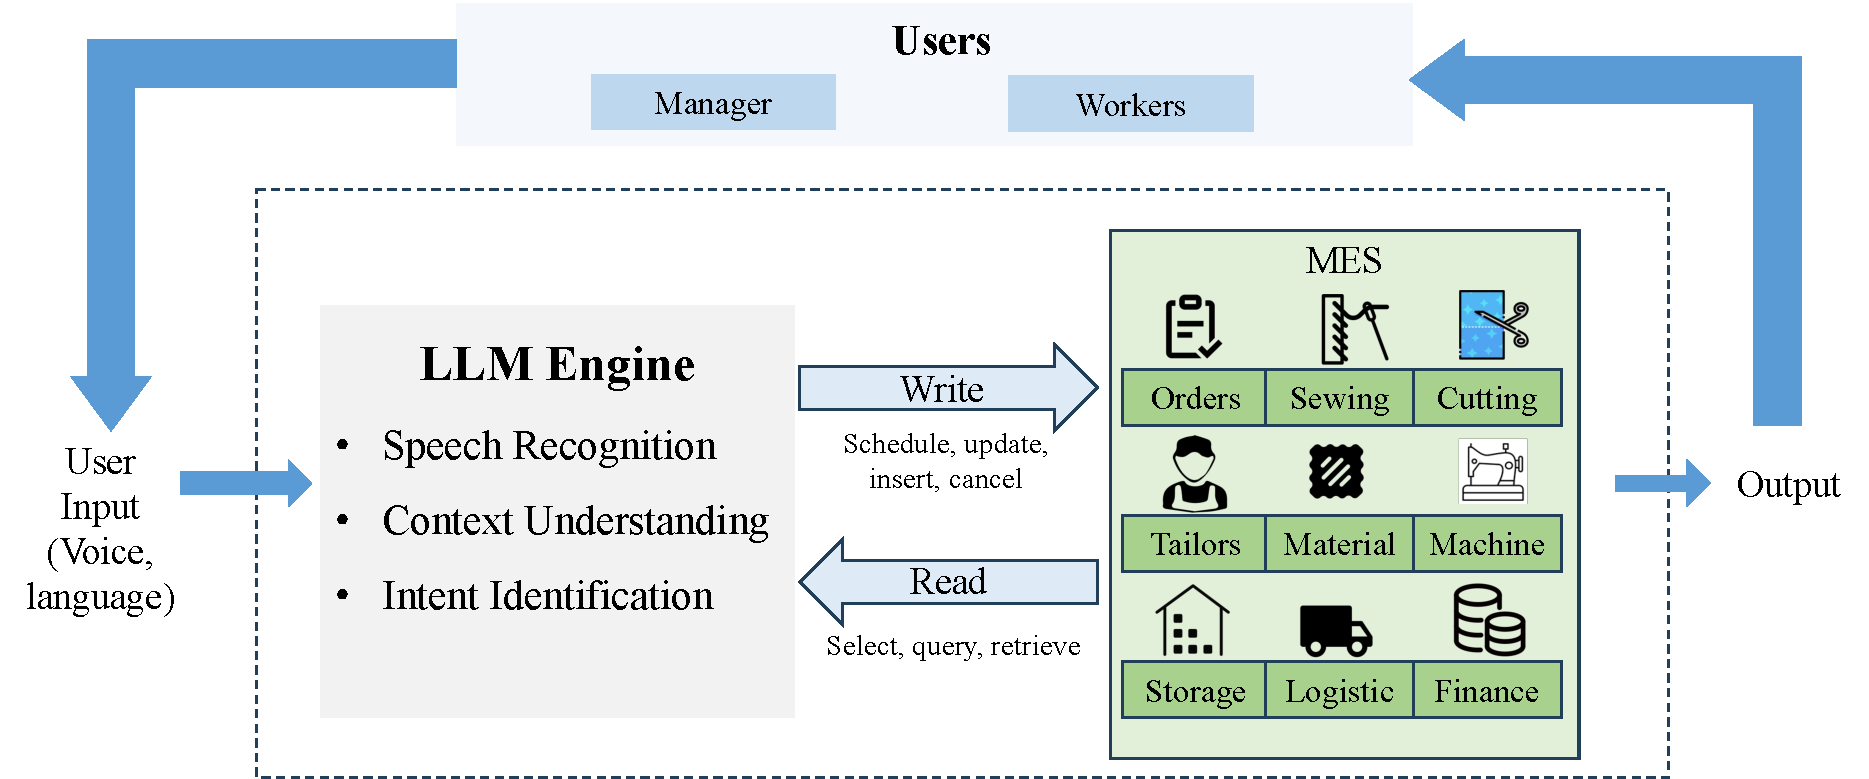
\includegraphics[width=\linewidth]{figs/functions.pdf}
% %% Use \caption command for figure caption and label.
% \caption{Figure Caption}\label{fig1}
% %% https://en.wikibooks.org/wiki/LaTeX/Importing_Graphics#Importing_external_graphics
% \end{figure}

 % balance between accuracy and token usage

 % Who should be responsible for wrong operations?

 % 
This study preliminarily implements a chatting interface of MES as a demonstration.
However, it is still far from being applicable in real factory settings and replacing the traditional GUI interfaces.
Three critical issues need to be discussed and addressed for future improvement.

\textbf{Balance between Accuracy, Generality, and Token usage}

Execution accuracy can be improved by designing more precise workflows or incorporating additional few-shot examples in prompts. However, this approach is akin to patching, which requires significant manpower and cannot be easily generalized to other MES systems. Additionally, complex workflows or lengthy prompts lead to high LLM token consumption.
% A more extensible 
The CWM is expected to evolve into a more extensible and dynamic framework that can understand database schema and production guidelines at a lower cost.

\textbf{Who should be responsible for incorrect operations?}

A typical MES requires a confirmation step before performing any data adjustment operations.
The operator who confirms the operation is responsible for any unforeseen consequences that may arise.
However, the CWM is a virtual worker who autonomously handles task planning and execution.
A critical issue in this process is determining the responsibility when the LLM performs unreasonable operations, even if the user provided correct instructions.
A viable solution is to incorporate a confirmation function in the chat window, where all details of the operations are clearly and thoroughly presented. 
Furthermore, it is meaningful to introduce counterfactual inference~\cite{del2024generating} to forecast the possible outcome under the hypothetical input requests.
Upon the user's affirmative "YES" during the confirmation phase, responsibility for the action and any outcomes is assumed by the user.

\textbf{Speaks little but is willing to express a lot.}
% A significant issue appears in our beta testing.
% In contrast to the traditional MES user interface, where developers can specify required fields for each submitted form, users of CWM are often reluctant to provide detailed operational information due to the unrestricted interaction mode.
In the traditional MES user interface, users must provide complete information in the submitted form, as input fields are typically set as mandatory by developers.
In CWM, the free interaction mode can lead users to become lax and inattentive in providing sufficient information.
The chatting agent has to keep inquiring about more information to complete the specified request, otherwise some vital information may be omitted during subsequent operation executions.
If we strictly limit the question options and required fields in CWM, the characteristic of free chatting is lost, and CWM will degenerate into a typical MES interaction model.
This dilemma inspires us to consider an important question, what is the best chatting interface for the CWM that is universally applicable, human-centered, and suitable for manufacturing environments?
% This quandary prompts us to consider a pivotal inquiry: what constitutes the optimal chat interface for the CWM that is universally applicable, human-centered, and tailored for industrial environments? As
As a preliminary feasibility study, the research utilizes Dify's basic chatting page as the interface.
However, there are many stakeholders for the CWM, including customers, production managers and workers.
The design of human-AI interfaces must take into their tasks, identities, and personas~\cite{holzinger2022personas}.
Designing next-generation human-AI interfaces for critical applications like manufacturing is crucial for the broader utilization of LLMs.
% subject that requires long-term exploration.



% In contrast to creative scenarios, serious scenarios rely heavily on workflow engineering~\cite{huang2024llmops} and are more challenging in product implementation.



\section{Conclusion}
\label{sec:conclusion}
This study proposes an LLM agent system, named Chat with MES (CWM), an interface for the operators in garment factories to manipulate a manufacturing execution system based on natural language.
We introduce two key technical innovations: the Request Re-writer and Multi-step Dynamic Operations Planning and Execution.
To eliminate entity ambiguity in the user's request, which may lead to incorrect query conditions, the Query Re-writer automatically aligns ambiguous entities in the users' input with the correct entities within the Manufacturing Execution System (MES), such as the names of customers, products, and materials.
To handle complicated manipulation requests on MES, the proposed Multi-step Dynamic Operations Planning and Execution combines the Text2SQL, LLM-Agents and Chain of Thoughts to plan a chain of basic operations and dynamically execute the operations step-by-step.
By evaluating the CWM on a simulated garment MES with 55 manually designed questions, we find that the CWM achieves a high execution success rate of 80\%, compared to GPT-4's 60\%. 
The query re-writer and Multi-step Dynamic Operations Planning and Execution techniques separately contribute improvements of approximately 10\% and 18\%, respectively.

In future study, we identify key areas for improvement, such as balancing execution accuracy and token usage, assigning responsibility for incorrect operations, and developing an optimal chatting interface for broad and human-centered applicability in manufacturing.

\section{Acknowledgment}
This research is partly supported by the Innovation and Technology Fund, China (No. PRP/015/24TI) and the Innovation and Technology Commission of the HKSAR Government through the InnoHK initiative."

% Based on a query re-writer, ambiguous entities in the customer's input are automatically aligned with the correct entities within the Manufacturing Execution System (MES), including customers, products, materials, and more.


% A case study conducted on a simulated garment MES with 50 artificial questions demonstrates the high execution accuracy of CWM (80\%) and the improvement brought by query re-writer (12.8\%) and Multi-Step Dynamic SQL generation (18.3\%). 


%% The Appendices part is started with the command \appendix;
%% appendix sections are then done as normal sections
% \appendix
% \section{Example Appendix Section}
% \label{app1}

% Appendix text.

% %% For citations use: 
% %%       \cite{<label>} ==> [1]

% %%
% Example citation, See \cite{lamport94}.

%% If you have bib database file and want bibtex to generate the
%% bibitems, please use
%%
 \bibliographystyle{elsarticle-num} 
 \bibliography{ref}

%% else use the following coding to input the bibitems directly in the
%% TeX file.

%% Refer following link for more details about bibliography and citations.
%% https://en.wikibooks.org/wiki/LaTeX/Bibliography_Management

% \begin{thebibliography}{00}

% %% For numbered reference style
% %% \bibitem{label}
% %% Text of bibliographic item

% \bibitem{lamport94}
%   Leslie Lamport,
%   \textit{\LaTeX: a document preparation system},
%   Addison Wesley, Massachusetts,
%   2nd edition,
%   1994.

% \end{thebibliography}
\end{document}

\endinput
%%
%% End of file `elsarticle-template-num.tex'.
